% Options for packages loaded elsewhere
\PassOptionsToPackage{unicode}{hyperref}
\PassOptionsToPackage{hyphens}{url}
%
\documentclass[
]{article}
\usepackage{amsmath,amssymb}
\usepackage{lmodern}
\usepackage{iftex}
\ifPDFTeX
  \usepackage[T1]{fontenc}
  \usepackage[utf8]{inputenc}
  \usepackage{textcomp} % provide euro and other symbols
\else % if luatex or xetex
  \usepackage{unicode-math}
  \defaultfontfeatures{Scale=MatchLowercase}
  \defaultfontfeatures[\rmfamily]{Ligatures=TeX,Scale=1}
\fi
% Use upquote if available, for straight quotes in verbatim environments
\IfFileExists{upquote.sty}{\usepackage{upquote}}{}
\IfFileExists{microtype.sty}{% use microtype if available
  \usepackage[]{microtype}
  \UseMicrotypeSet[protrusion]{basicmath} % disable protrusion for tt fonts
}{}
\makeatletter
\@ifundefined{KOMAClassName}{% if non-KOMA class
  \IfFileExists{parskip.sty}{%
    \usepackage{parskip}
  }{% else
    \setlength{\parindent}{0pt}
    \setlength{\parskip}{6pt plus 2pt minus 1pt}}
}{% if KOMA class
  \KOMAoptions{parskip=half}}
\makeatother
\usepackage{xcolor}
\usepackage[margin=1in]{geometry}
\usepackage{color}
\usepackage{fancyvrb}
\newcommand{\VerbBar}{|}
\newcommand{\VERB}{\Verb[commandchars=\\\{\}]}
\DefineVerbatimEnvironment{Highlighting}{Verbatim}{commandchars=\\\{\}}
% Add ',fontsize=\small' for more characters per line
\usepackage{framed}
\definecolor{shadecolor}{RGB}{248,248,248}
\newenvironment{Shaded}{\begin{snugshade}}{\end{snugshade}}
\newcommand{\AlertTok}[1]{\textcolor[rgb]{0.94,0.16,0.16}{#1}}
\newcommand{\AnnotationTok}[1]{\textcolor[rgb]{0.56,0.35,0.01}{\textbf{\textit{#1}}}}
\newcommand{\AttributeTok}[1]{\textcolor[rgb]{0.77,0.63,0.00}{#1}}
\newcommand{\BaseNTok}[1]{\textcolor[rgb]{0.00,0.00,0.81}{#1}}
\newcommand{\BuiltInTok}[1]{#1}
\newcommand{\CharTok}[1]{\textcolor[rgb]{0.31,0.60,0.02}{#1}}
\newcommand{\CommentTok}[1]{\textcolor[rgb]{0.56,0.35,0.01}{\textit{#1}}}
\newcommand{\CommentVarTok}[1]{\textcolor[rgb]{0.56,0.35,0.01}{\textbf{\textit{#1}}}}
\newcommand{\ConstantTok}[1]{\textcolor[rgb]{0.00,0.00,0.00}{#1}}
\newcommand{\ControlFlowTok}[1]{\textcolor[rgb]{0.13,0.29,0.53}{\textbf{#1}}}
\newcommand{\DataTypeTok}[1]{\textcolor[rgb]{0.13,0.29,0.53}{#1}}
\newcommand{\DecValTok}[1]{\textcolor[rgb]{0.00,0.00,0.81}{#1}}
\newcommand{\DocumentationTok}[1]{\textcolor[rgb]{0.56,0.35,0.01}{\textbf{\textit{#1}}}}
\newcommand{\ErrorTok}[1]{\textcolor[rgb]{0.64,0.00,0.00}{\textbf{#1}}}
\newcommand{\ExtensionTok}[1]{#1}
\newcommand{\FloatTok}[1]{\textcolor[rgb]{0.00,0.00,0.81}{#1}}
\newcommand{\FunctionTok}[1]{\textcolor[rgb]{0.00,0.00,0.00}{#1}}
\newcommand{\ImportTok}[1]{#1}
\newcommand{\InformationTok}[1]{\textcolor[rgb]{0.56,0.35,0.01}{\textbf{\textit{#1}}}}
\newcommand{\KeywordTok}[1]{\textcolor[rgb]{0.13,0.29,0.53}{\textbf{#1}}}
\newcommand{\NormalTok}[1]{#1}
\newcommand{\OperatorTok}[1]{\textcolor[rgb]{0.81,0.36,0.00}{\textbf{#1}}}
\newcommand{\OtherTok}[1]{\textcolor[rgb]{0.56,0.35,0.01}{#1}}
\newcommand{\PreprocessorTok}[1]{\textcolor[rgb]{0.56,0.35,0.01}{\textit{#1}}}
\newcommand{\RegionMarkerTok}[1]{#1}
\newcommand{\SpecialCharTok}[1]{\textcolor[rgb]{0.00,0.00,0.00}{#1}}
\newcommand{\SpecialStringTok}[1]{\textcolor[rgb]{0.31,0.60,0.02}{#1}}
\newcommand{\StringTok}[1]{\textcolor[rgb]{0.31,0.60,0.02}{#1}}
\newcommand{\VariableTok}[1]{\textcolor[rgb]{0.00,0.00,0.00}{#1}}
\newcommand{\VerbatimStringTok}[1]{\textcolor[rgb]{0.31,0.60,0.02}{#1}}
\newcommand{\WarningTok}[1]{\textcolor[rgb]{0.56,0.35,0.01}{\textbf{\textit{#1}}}}
\usepackage{graphicx}
\makeatletter
\def\maxwidth{\ifdim\Gin@nat@width>\linewidth\linewidth\else\Gin@nat@width\fi}
\def\maxheight{\ifdim\Gin@nat@height>\textheight\textheight\else\Gin@nat@height\fi}
\makeatother
% Scale images if necessary, so that they will not overflow the page
% margins by default, and it is still possible to overwrite the defaults
% using explicit options in \includegraphics[width, height, ...]{}
\setkeys{Gin}{width=\maxwidth,height=\maxheight,keepaspectratio}
% Set default figure placement to htbp
\makeatletter
\def\fps@figure{htbp}
\makeatother
\setlength{\emergencystretch}{3em} % prevent overfull lines
\providecommand{\tightlist}{%
  \setlength{\itemsep}{0pt}\setlength{\parskip}{0pt}}
\setcounter{secnumdepth}{-\maxdimen} % remove section numbering
\usepackage{booktabs}
\usepackage{longtable}
\usepackage{array}
\usepackage{multirow}
\usepackage{wrapfig}
\usepackage{float}
\usepackage{colortbl}
\usepackage{pdflscape}
\usepackage{tabu}
\usepackage{threeparttable}
\usepackage{threeparttablex}
\usepackage[normalem]{ulem}
\usepackage{makecell}
\usepackage{xcolor}
\ifLuaTeX
  \usepackage{selnolig}  % disable illegal ligatures
\fi
\IfFileExists{bookmark.sty}{\usepackage{bookmark}}{\usepackage{hyperref}}
\IfFileExists{xurl.sty}{\usepackage{xurl}}{} % add URL line breaks if available
\urlstyle{same} % disable monospaced font for URLs
\hypersetup{
  pdftitle={Assignemnt 1},
  pdfauthor={Anne Valder},
  hidelinks,
  pdfcreator={LaTeX via pandoc}}

\title{Assignemnt 1}
\author{Anne Valder}
\date{2023-11-09}

\begin{document}
\maketitle

\hypertarget{tasks}{%
\section{Tasks}\label{tasks}}

\begin{enumerate}
\def\labelenumi{\arabic{enumi}.}
\item
  Build four predictive models using linear regression for earnings per
  hour. The target variable is earnings per hour, all others would be
  predictors.Model 1 shall be the simplest, model 4 the more complex. It
  shall be OLS. You shall explain your choice of predictors.
\item
  Compare model performance of these models (a) RMSE in the full sample,
  (2) cross-validated RMSE and (c) BIC in the full sample.
\item
  Discuss the relationship between model complexity and performance. You
  may use visual aids.
\end{enumerate}

\begin{verbatim}
## [1] "C:/Users/avalder/OneDrive - WU Wien/Documents/Study/WS_23_24/Pred_MLE_Econ/da_case_studies"
\end{verbatim}

\begin{verbatim}
## Warning: Paket 'tidyverse' wurde unter R Version 4.3.1 erstellt
\end{verbatim}

\begin{verbatim}
## Warning: Paket 'ggplot2' wurde unter R Version 4.3.1 erstellt
\end{verbatim}

\begin{verbatim}
## Warning: Paket 'tibble' wurde unter R Version 4.3.1 erstellt
\end{verbatim}

\begin{verbatim}
## Warning: Paket 'tidyr' wurde unter R Version 4.3.1 erstellt
\end{verbatim}

\begin{verbatim}
## Warning: Paket 'readr' wurde unter R Version 4.3.1 erstellt
\end{verbatim}

\begin{verbatim}
## Warning: Paket 'purrr' wurde unter R Version 4.3.1 erstellt
\end{verbatim}

\begin{verbatim}
## Warning: Paket 'dplyr' wurde unter R Version 4.3.1 erstellt
\end{verbatim}

\begin{verbatim}
## Warning: Paket 'stringr' wurde unter R Version 4.3.1 erstellt
\end{verbatim}

\begin{verbatim}
## Warning: Paket 'forcats' wurde unter R Version 4.3.1 erstellt
\end{verbatim}

\begin{verbatim}
## Warning: Paket 'lubridate' wurde unter R Version 4.3.1 erstellt
\end{verbatim}

\begin{verbatim}
## -- Attaching core tidyverse packages ------------------------ tidyverse 2.0.0 --
## v dplyr     1.1.3     v readr     2.1.4
## v forcats   1.0.0     v stringr   1.5.0
## v ggplot2   3.4.4     v tibble    3.2.1
## v lubridate 1.9.3     v tidyr     1.3.0
## v purrr     1.0.2     
## -- Conflicts ------------------------------------------ tidyverse_conflicts() --
## x dplyr::filter() masks stats::filter()
## x dplyr::lag()    masks stats::lag()
## i Use the conflicted package (<http://conflicted.r-lib.org/>) to force all conflicts to become errors
\end{verbatim}

\begin{verbatim}
## Warning: Paket 'scales' wurde unter R Version 4.3.1 erstellt
\end{verbatim}

\begin{verbatim}
## 
## Attache Paket: 'scales'
## 
## Das folgende Objekt ist maskiert 'package:purrr':
## 
##     discard
## 
## Das folgende Objekt ist maskiert 'package:readr':
## 
##     col_factor
\end{verbatim}

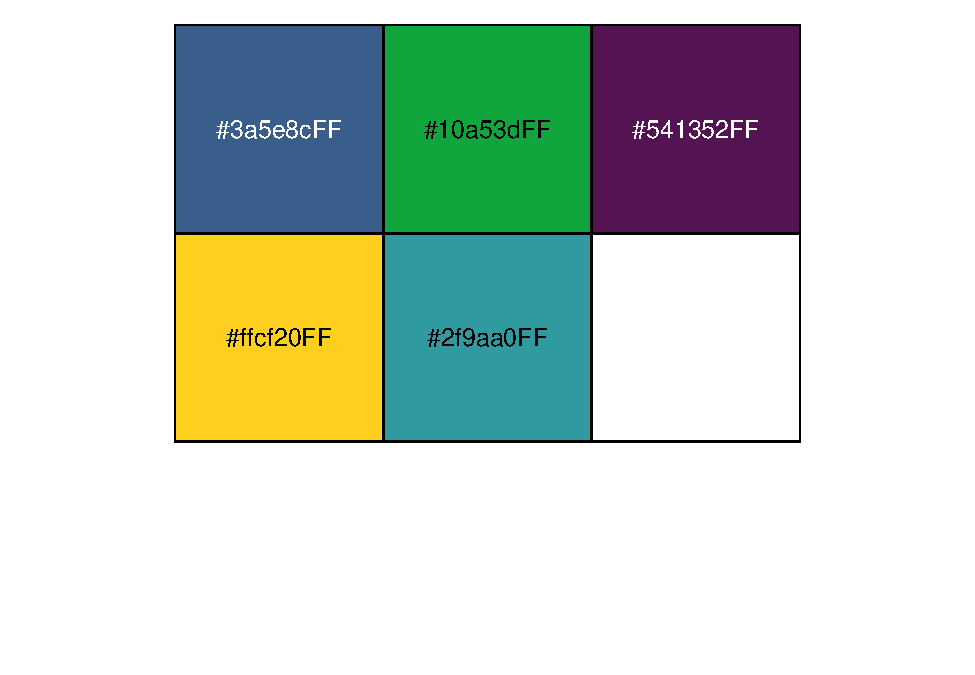
\includegraphics{A1_files/figure-latex/unnamed-chunk-2-1.pdf}

\begin{verbatim}
## Warning: Paket 'urca' wurde unter R Version 4.3.1 erstellt
\end{verbatim}

\begin{verbatim}
## Warning: Paket 'stargazer' wurde unter R Version 4.3.1 erstellt
\end{verbatim}

\begin{verbatim}
## 
## Please cite as: 
## 
##  Hlavac, Marek (2022). stargazer: Well-Formatted Regression and Summary Statistics Tables.
##  R package version 5.2.3. https://CRAN.R-project.org/package=stargazer
\end{verbatim}

\begin{verbatim}
## Warning: Paket 'sandwich' wurde unter R Version 4.3.1 erstellt
\end{verbatim}

\begin{verbatim}
## Warning: Paket 'Metrics' wurde unter R Version 4.3.2 erstellt
\end{verbatim}

\begin{verbatim}
## Warning: Paket 'caret' wurde unter R Version 4.3.2 erstellt
\end{verbatim}

\begin{verbatim}
## Lade nötiges Paket: lattice
\end{verbatim}

\begin{verbatim}
## 
## Attache Paket: 'caret'
\end{verbatim}

\begin{verbatim}
## Die folgenden Objekte sind maskiert von 'package:Metrics':
## 
##     precision, recall
\end{verbatim}

\begin{verbatim}
## Das folgende Objekt ist maskiert 'package:purrr':
## 
##     lift
\end{verbatim}

\begin{verbatim}
## Warning: Paket 'modelsummary' wurde unter R Version 4.3.2 erstellt
\end{verbatim}

\begin{verbatim}
## Warning: Paket 'fixest' wurde unter R Version 4.3.2 erstellt
\end{verbatim}

\begin{verbatim}
## 
## Attache Paket: 'fixest'
\end{verbatim}

\begin{verbatim}
## Das folgende Objekt ist maskiert durch '.GlobalEnv':
## 
##     d
\end{verbatim}

\begin{verbatim}
## Das folgende Objekt ist maskiert 'package:Metrics':
## 
##     se
\end{verbatim}

\begin{verbatim}
## Das folgende Objekt ist maskiert 'package:scales':
## 
##     pvalue
\end{verbatim}

\begin{verbatim}
## Warning: Paket 'lmtest' wurde unter R Version 4.3.2 erstellt
\end{verbatim}

\begin{verbatim}
## Lade nötiges Paket: zoo
\end{verbatim}

\begin{verbatim}
## Warning: Paket 'zoo' wurde unter R Version 4.3.1 erstellt
\end{verbatim}

\begin{verbatim}
## 
## Attache Paket: 'zoo'
\end{verbatim}

\begin{verbatim}
## Die folgenden Objekte sind maskiert von 'package:base':
## 
##     as.Date, as.Date.numeric
\end{verbatim}

\begin{verbatim}
## New names:
## * `` -> `...1`
\end{verbatim}

\hypertarget{data-preperations-first-filtering-for-occupation-2310---elementary-and-middle-school-teachers}{%
\subsubsection{Data preperations (first filtering for occupation: 2310 -
elementary and middle school
teachers)}\label{data-preperations-first-filtering-for-occupation-2310---elementary-and-middle-school-teachers}}

\hypertarget{e.g.-research-question-predictions-might-help-you-to-decide-what-salary-to-put-in-a-job-ad-for-teachers.-or-what-are-the-differences-between-female-and-male-salaries.-are-there-differences-between-government-and-private-employees-regarding-the-salary}{%
\paragraph{e.g.~Research question: Predictions might help you to decide
what salary to put in a job ad for teachers. Or what are the differences
between female and male salaries. Are there differences between
government and private employees regarding the
salary?}\label{e.g.-research-question-predictions-might-help-you-to-decide-what-salary-to-put-in-a-job-ad-for-teachers.-or-what-are-the-differences-between-female-and-male-salaries.-are-there-differences-between-government-and-private-employees-regarding-the-salary}}

\begin{Shaded}
\begin{Highlighting}[]
\NormalTok{data }\OtherTok{\textless{}{-}}\NormalTok{ data\_all }\SpecialCharTok{\%\textgreater{}\%} \FunctionTok{filter}\NormalTok{(occ2012 }\SpecialCharTok{==} \DecValTok{2310}\NormalTok{)  }\CommentTok{\#Elementary and middle school teachers}

\FunctionTok{summary}\NormalTok{(data)}
\end{Highlighting}
\end{Shaded}

\begin{verbatim}
##       ...1             hhid             intmonth            stfips         
##  Min.   :    43   Min.   :8.172e+09   Length:3636        Length:3636       
##  1st Qu.: 79668   1st Qu.:1.409e+14   Class :character   Class :character  
##  Median :161147   Median :4.104e+14   Mode  :character   Mode  :character  
##  Mean   :159810   Mean   :4.481e+14                                        
##  3rd Qu.:241508   3rd Qu.:7.220e+14                                        
##  Max.   :317003   Max.   :9.998e+14                                        
##                                                                            
##      weight            earnwke            uhours         grade92     
##  Min.   :   65.99   Min.   :   0.23   Min.   : 1.00   Min.   :34.00  
##  1st Qu.: 1217.92   1st Qu.: 692.30   1st Qu.:40.00   1st Qu.:43.00  
##  Median : 2655.19   Median : 961.00   Median :40.00   Median :43.00  
##  Mean   : 2317.61   Mean   :1034.20   Mean   :40.69   Mean   :43.31  
##  3rd Qu.: 3279.23   3rd Qu.:1250.00   3rd Qu.:40.00   3rd Qu.:44.00  
##  Max.   :10672.16   Max.   :2884.61   Max.   :80.00   Max.   :46.00  
##                                                                      
##       race            ethnic           age             sex      
##  Min.   : 1.000   Min.   :1.000   Min.   :16.00   Min.   :1.00  
##  1st Qu.: 1.000   1st Qu.:1.000   1st Qu.:33.00   1st Qu.:2.00  
##  Median : 1.000   Median :1.000   Median :42.00   Median :2.00  
##  Mean   : 1.278   Mean   :2.567   Mean   :42.16   Mean   :1.82  
##  3rd Qu.: 1.000   3rd Qu.:3.000   3rd Qu.:51.00   3rd Qu.:2.00  
##  Max.   :21.000   Max.   :8.000   Max.   :64.00   Max.   :2.00  
##                   NA's   :3375                                  
##     marital         ownchild         chldpres       prcitshp        
##  Min.   :1.000   Min.   :0.0000   Min.   : 0.00   Length:3636       
##  1st Qu.:1.000   1st Qu.:0.0000   1st Qu.: 0.00   Class :character  
##  Median :1.000   Median :0.0000   Median : 0.00   Mode  :character  
##  Mean   :2.536   Mean   :0.8839   Mean   : 2.36                     
##  3rd Qu.:5.000   3rd Qu.:2.0000   3rd Qu.: 4.00                     
##  Max.   :7.000   Max.   :9.0000   Max.   :15.00                     
##                                                                     
##     state              ind02              occ2012        class          
##  Length:3636        Length:3636        Min.   :2310   Length:3636       
##  Class :character   Class :character   1st Qu.:2310   Class :character  
##  Mode  :character   Mode  :character   Median :2310   Mode  :character  
##                                        Mean   :2310                     
##                                        3rd Qu.:2310                     
##                                        Max.   :2310                     
##                                                                         
##    unionmme           unioncov            lfsr94         
##  Length:3636        Length:3636        Length:3636       
##  Class :character   Class :character   Class :character  
##  Mode  :character   Mode  :character   Mode  :character  
##                                                          
##                                                          
##                                                          
## 
\end{verbatim}

\begin{Shaded}
\begin{Highlighting}[]
\FunctionTok{glimpse}\NormalTok{ (data)}
\end{Highlighting}
\end{Shaded}

\begin{verbatim}
## Rows: 3,636
## Columns: 23
## $ ...1     <dbl> 43, 55, 116, 199, 286, 324, 325, 367, 378, 401, 404, 433, 486~
## $ hhid     <dbl> 9.540019e+14, 9.817093e+14, 3.103431e+14, 6.780120e+14, 2.437~
## $ intmonth <chr> "January", "January", "January", "January", "January", "Janua~
## $ stfips   <chr> "AL", "AL", "AL", "AL", "AK", "AK", "AK", "AK", "AK", "AK", "~
## $ weight   <dbl> 2847.5801, 3102.3708, 2690.8661, 2424.1925, 341.9676, 414.704~
## $ earnwke  <dbl> 826.92, 68.00, 673.07, 1000.00, 520.00, 769.23, 1115.38, 1346~
## $ uhours   <dbl> 40, 8, 45, 56, 40, 50, 50, 70, 40, 40, 45, 55, 20, 45, 16, 40~
## $ grade92  <dbl> 44, 40, 43, 44, 39, 43, 43, 43, 40, 44, 39, 43, 43, 43, 44, 4~
## $ race     <dbl> 1, 1, 1, 2, 1, 1, 1, 1, 2, 1, 1, 1, 1, 1, 1, 1, 1, 1, 1, 2, 2~
## $ ethnic   <dbl> NA, NA, NA, NA, NA, NA, NA, NA, NA, NA, NA, NA, NA, NA, NA, N~
## $ age      <dbl> 31, 21, 39, 57, 45, 32, 35, 56, 56, 25, 33, 25, 53, 24, 63, 5~
## $ sex      <dbl> 2, 2, 2, 2, 2, 2, 1, 2, 2, 2, 2, 2, 1, 2, 2, 2, 2, 1, 1, 2, 2~
## $ marital  <dbl> 7, 1, 1, 7, 1, 1, 1, 1, 7, 7, 1, 1, 5, 7, 1, 1, 5, 1, 1, 5, 7~
## $ ownchild <dbl> 0, 0, 0, 0, 2, 2, 2, 0, 0, 0, 3, 1, 0, 0, 0, 0, 0, 0, 0, 1, 0~
## $ chldpres <dbl> 0, 0, 0, 0, 9, 5, 5, 0, 0, 0, 4, 2, 0, 0, 0, 0, 0, 0, 0, 4, 0~
## $ prcitshp <chr> "Native, Born In US", "Native, Born In US", "Native, Born In ~
## $ state    <chr> "63", "63", "63", "63", "94", "94", "94", "94", "94", "94", "~
## $ ind02    <chr> "Elementary and secondary schools (6111)", "Elementary and se~
## $ occ2012  <dbl> 2310, 2310, 2310, 2310, 2310, 2310, 2310, 2310, 2310, 2310, 2~
## $ class    <chr> "Private, For Profit", "Private, For Profit", "Government - L~
## $ unionmme <chr> "No", "No", "Yes", "Yes", "Yes", "Yes", "Yes", "Yes", "Yes", ~
## $ unioncov <chr> "No", "No", NA, NA, NA, NA, NA, NA, NA, NA, NA, "No", NA, NA,~
## $ lfsr94   <chr> "Employed-At Work", "Employed-At Work", "Employed-At Work", "~
\end{verbatim}

\hypertarget{sample-design-filtering-the-data-to-match-the-business-policy-question.}{%
\subsubsection{Sample design: filtering the data to match the business/
policy
question.}\label{sample-design-filtering-the-data-to-match-the-business-policy-question.}}

\begin{Shaded}
\begin{Highlighting}[]
\CommentTok{\# 1) construct the target variable earnings per hour from \textquotesingle{}weekly earnings\textquotesingle{} and \textquotesingle{}usual work hours\textquotesingle{}:}

\NormalTok{data }\OtherTok{\textless{}{-}}\NormalTok{ data }\SpecialCharTok{\%\textgreater{}\%} \FunctionTok{mutate}\NormalTok{(}\AttributeTok{earnh=}\NormalTok{earnwke}\SpecialCharTok{/}\NormalTok{uhours)}

                         
\CommentTok{\# 2) drop extreme values where earning per hour is below 1 or larger than 300. We are interested in predicting "standard" teaching salaries.Salaries smaller than 1 would be considered errors in our case. Keeping an extreme value like \textquotesingle{}583\textquotesingle{} that is likely to be an error, will have a high cost {-} the quadratic errors in the loss function will tilt the curve and our prediction will be off for most observations.}

\NormalTok{data }\SpecialCharTok{\%\textgreater{}\%}\NormalTok{ dplyr}\SpecialCharTok{::}\FunctionTok{select}\NormalTok{(earnh) }\SpecialCharTok{\%\textgreater{}\%} \FunctionTok{summary}\NormalTok{()}
\end{Highlighting}
\end{Shaded}

\begin{verbatim}
##      earnh         
##  Min.   :  0.0041  
##  1st Qu.: 16.8268  
##  Median : 23.0768  
##  Mean   : 25.9114  
##  3rd Qu.: 31.2500  
##  Max.   :583.3300
\end{verbatim}

\begin{Shaded}
\begin{Highlighting}[]
\NormalTok{data }\OtherTok{\textless{}{-}}\NormalTok{ data }\SpecialCharTok{\%\textgreater{}\%} \FunctionTok{filter}\NormalTok{(earnh }\SpecialCharTok{\textgreater{}=} \DecValTok{1} \SpecialCharTok{\&}\NormalTok{ earnh }\SpecialCharTok{\textless{}=} \DecValTok{300}\NormalTok{)}

\CommentTok{\# 3) select age range of working population (18{-}65) as we want to predict a competitive teacher salary (here also a proxy for teachers working full time / main job)}

\NormalTok{data }\SpecialCharTok{\%\textgreater{}\%}\NormalTok{ dplyr}\SpecialCharTok{::}\FunctionTok{select}\NormalTok{(age) }\SpecialCharTok{\%\textgreater{}\%} \FunctionTok{summary}\NormalTok{()}
\end{Highlighting}
\end{Shaded}

\begin{verbatim}
##       age       
##  Min.   :16.00  
##  1st Qu.:33.00  
##  Median :42.00  
##  Mean   :42.16  
##  3rd Qu.:51.00  
##  Max.   :64.00
\end{verbatim}

\begin{Shaded}
\begin{Highlighting}[]
\CommentTok{\#summary(as.factor(data$age))}

\NormalTok{data }\OtherTok{\textless{}{-}}\NormalTok{ data }\SpecialCharTok{\%\textgreater{}\%} \FunctionTok{filter}\NormalTok{(age }\SpecialCharTok{\textgreater{}=} \DecValTok{18} \SpecialCharTok{\&}\NormalTok{ earnh }\SpecialCharTok{\textless{}=} \DecValTok{65}\NormalTok{)}

\CommentTok{\# 4) Only consider teachers with a certain level of education (we do not want to include for example tutoring from high school students when predicting a standard competitive teacher salary. Thus we restrict the sample to people who have a High school graduate, diploma or GED (i.e. grade92 \textgreater{}= 38)  }

\CommentTok{\# variable grade 92: Highest grade attended}
\CommentTok{\#34 7th or 8th}
\CommentTok{\#36 10th }
\CommentTok{\#37 11th}
\CommentTok{\#38 12th grade NO DIPLOMA}
\CommentTok{\#39 High school graduate, diploma or GED START }
\CommentTok{\#40 Some college but no degree }
\CommentTok{\#41 Associate degree {-}{-} occupational/vocational }
\CommentTok{\#42 Associate degree {-}{-} academic program }
\CommentTok{\#43 Bachelor\textquotesingle{}s degree (e.g. BA,AB,BS) }
\CommentTok{\#44 Master\textquotesingle{}s degree (e.g. MA,MS,MEng,Med,MSW,MBA) }
\CommentTok{\#45 Professional school deg. (e.g. MD,DDS,DVM,LLB,JD)}
\CommentTok{\#46 Doctorate degree (e.g. PhD, EdD) }

\FunctionTok{summary}\NormalTok{(}\FunctionTok{as.factor}\NormalTok{(data}\SpecialCharTok{$}\NormalTok{grade92))}
\end{Highlighting}
\end{Shaded}

\begin{verbatim}
##   34   36   37   38   39   40   41   42   43   44   45   46 
##    1    1    3    5   72  103   31   66 1521 1671   46   39
\end{verbatim}

\begin{Shaded}
\begin{Highlighting}[]
\NormalTok{data }\OtherTok{\textless{}{-}}\NormalTok{ data }\SpecialCharTok{\%\textgreater{}\%} \FunctionTok{filter}\NormalTok{(grade92 }\SpecialCharTok{\textgreater{}=} \DecValTok{38}\NormalTok{)}


\FunctionTok{summary}\NormalTok{(}\FunctionTok{as.factor}\NormalTok{(data}\SpecialCharTok{$}\NormalTok{ind02)) }\CommentTok{\# all TRUE }
\end{Highlighting}
\end{Shaded}

\begin{verbatim}
## Elementary and secondary schools (6111) 
##                                    3554
\end{verbatim}

\hypertarget{visualize-data}{%
\subsubsection{visualize data}\label{visualize-data}}

\begin{Shaded}
\begin{Highlighting}[]
\CommentTok{\# distribution of earnings per hour }


\NormalTok{hist\_earnh }\OtherTok{\textless{}{-}} \FunctionTok{ggplot}\NormalTok{(data, }\FunctionTok{aes}\NormalTok{(}\AttributeTok{x=}\NormalTok{earnh))}\SpecialCharTok{+}
              \FunctionTok{geom\_histogram}\NormalTok{(}\AttributeTok{binwidth =} \DecValTok{2}\NormalTok{, }\AttributeTok{fill =}\NormalTok{ color[}\DecValTok{1}\NormalTok{], }\AttributeTok{color =}\NormalTok{ color.outline, }
                             \AttributeTok{alpha =} \FloatTok{0.8}\NormalTok{, }\AttributeTok{size =} \FloatTok{0.25}\NormalTok{) }\SpecialCharTok{+}
              \FunctionTok{ylab}\NormalTok{(}\StringTok{"Count"}\NormalTok{) }\SpecialCharTok{+}
              \FunctionTok{xlab}\NormalTok{(}\StringTok{"Earnings per hour"}\NormalTok{) }\SpecialCharTok{+}
              \FunctionTok{theme\_bg}\NormalTok{()}
\end{Highlighting}
\end{Shaded}

\begin{verbatim}
## Warning: Using `size` aesthetic for lines was deprecated in ggplot2 3.4.0.
## i Please use `linewidth` instead.
## This warning is displayed once every 8 hours.
## Call `lifecycle::last_lifecycle_warnings()` to see where this warning was
## generated.
\end{verbatim}

\begin{verbatim}
## Warning: The `size` argument of `element_rect()` is deprecated as of ggplot2 3.4.0.
## i Please use the `linewidth` argument instead.
## This warning is displayed once every 8 hours.
## Call `lifecycle::last_lifecycle_warnings()` to see where this warning was
## generated.
\end{verbatim}

\begin{verbatim}
## Warning: The `size` argument of `element_line()` is deprecated as of ggplot2 3.4.0.
## i Please use the `linewidth` argument instead.
## This warning is displayed once every 8 hours.
## Call `lifecycle::last_lifecycle_warnings()` to see where this warning was
## generated.
\end{verbatim}

\begin{Shaded}
\begin{Highlighting}[]
\NormalTok{hist\_earnh}
\end{Highlighting}
\end{Shaded}

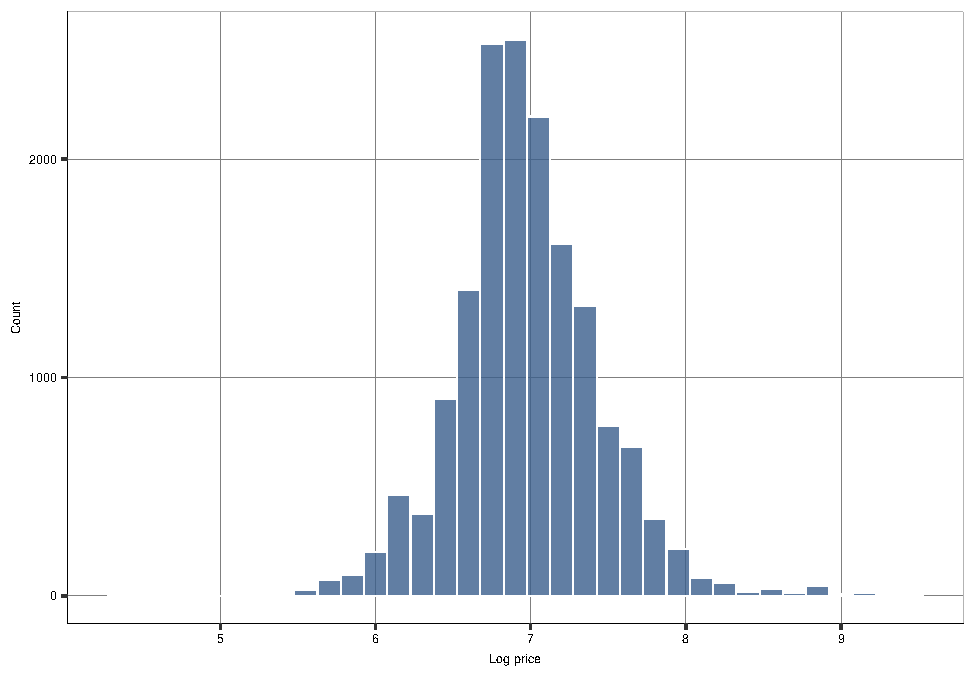
\includegraphics{A1_files/figure-latex/unnamed-chunk-7-1.pdf}

\hypertarget{label-engineering}{%
\subsubsection{label engineering}\label{label-engineering}}

\begin{Shaded}
\begin{Highlighting}[]
\DocumentationTok{\#\#\# label engineering: log vs label, otherwise given:}
\CommentTok{\# Use when: More interested in relative changes than in changes per currency. Log differences approximate relative, or percentage, differences, and relative price differences are often more stable.The related technical advantage is that the distribution of log prices is often close to normal, which makes linear regressions give better approximation to average differences.}

\CommentTok{\#do:Look at some patterns \& Compare model performance}

\NormalTok{data }\OtherTok{\textless{}{-}}\NormalTok{ data }\SpecialCharTok{\%\textgreater{}\%} \FunctionTok{mutate}\NormalTok{(}\AttributeTok{learnh=}\FunctionTok{log}\NormalTok{(earnh))}


\NormalTok{hist\_learnh }\OtherTok{\textless{}{-}} \FunctionTok{ggplot}\NormalTok{(data, }\FunctionTok{aes}\NormalTok{(}\AttributeTok{x=}\NormalTok{learnh))}\SpecialCharTok{+}
              \FunctionTok{geom\_histogram}\NormalTok{(}\AttributeTok{binwidth =} \FloatTok{0.1}\NormalTok{, }\AttributeTok{fill =}\NormalTok{ color[}\DecValTok{1}\NormalTok{], }\AttributeTok{color =}\NormalTok{color.outline, }\AttributeTok{alpha =} \FloatTok{0.8}\NormalTok{, }\AttributeTok{size =} \FloatTok{0.25}\NormalTok{) }\SpecialCharTok{+}
              \FunctionTok{ylab}\NormalTok{(}\StringTok{"Count"}\NormalTok{) }\SpecialCharTok{+}
              \FunctionTok{xlab}\NormalTok{(}\StringTok{"Earnings per hour (log)"}\NormalTok{) }\SpecialCharTok{+}
              \FunctionTok{theme\_bg}\NormalTok{()}

\NormalTok{hist\_learnh}
\end{Highlighting}
\end{Shaded}

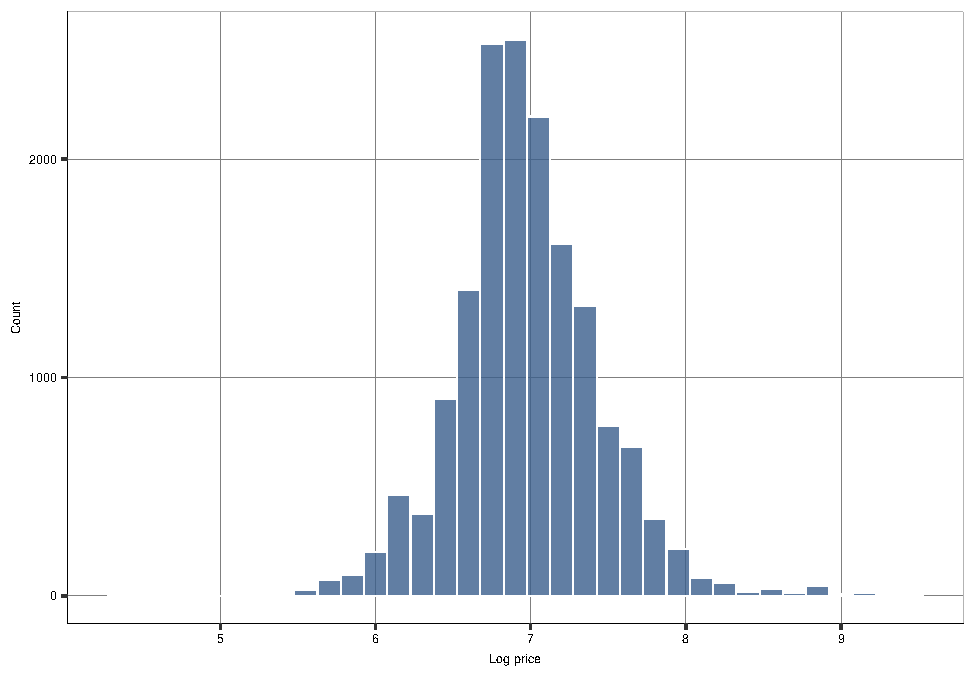
\includegraphics{A1_files/figure-latex/unnamed-chunk-8-1.pdf}

\begin{Shaded}
\begin{Highlighting}[]
\CommentTok{\# levels seems to be fine here }
\end{Highlighting}
\end{Shaded}

\hypertarget{feature-engineering}{%
\subsection{feature engineering}\label{feature-engineering}}

\hypertarget{missing-values}{%
\subsubsection{1) missing values}\label{missing-values}}

\begin{Shaded}
\begin{Highlighting}[]
\CommentTok{\#1. What to do with missing values? }

\CommentTok{\# where do we have missing variables in our data se?}
\NormalTok{to\_filter }\OtherTok{\textless{}{-}} \FunctionTok{sapply}\NormalTok{(data, }\ControlFlowTok{function}\NormalTok{(x) }\FunctionTok{sum}\NormalTok{(}\FunctionTok{is.na}\NormalTok{(x)))}
\NormalTok{to\_filter[to\_filter }\SpecialCharTok{\textgreater{}} \DecValTok{0}\NormalTok{]}
\end{Highlighting}
\end{Shaded}

\begin{verbatim}
##   ethnic unioncov 
##     3299     1827
\end{verbatim}

\begin{Shaded}
\begin{Highlighting}[]
\NormalTok{data}\SpecialCharTok{$}\NormalTok{ethnic }\OtherTok{\textless{}{-}} \FunctionTok{fct\_explicit\_na}\NormalTok{(}\FunctionTok{as.character}\NormalTok{(data}\SpecialCharTok{$}\NormalTok{ethnic),}\AttributeTok{na\_level =} \StringTok{"Missing"}\NormalTok{)}
\end{Highlighting}
\end{Shaded}

\begin{verbatim}
## Warning: `fct_explicit_na()` was deprecated in forcats 1.0.0.
## i Please use `fct_na_value_to_level()` instead.
## This warning is displayed once every 8 hours.
## Call `lifecycle::last_lifecycle_warnings()` to see where this warning was
## generated.
\end{verbatim}

\begin{Shaded}
\begin{Highlighting}[]
\NormalTok{data}\SpecialCharTok{$}\NormalTok{unioncov  }\OtherTok{\textless{}{-}} \FunctionTok{fct\_explicit\_na}\NormalTok{(data}\SpecialCharTok{$}\NormalTok{unioncov ,}\AttributeTok{na\_level =} \StringTok{"Missing"}\NormalTok{)}

\CommentTok{\#ethnic, use race instead}
\CommentTok{\#union cov, use unionmme instead {-} so no imputations necessary}
\end{Highlighting}
\end{Shaded}

\hypertarget{ordered-categorical-values-text-binary-variables}{%
\subsubsection{2) \& 3) ordered categorical values, text, binary
variables}\label{ordered-categorical-values-text-binary-variables}}

\#2. Dealing with ordered categorical values - continuous or set of
binaries \#If binary (e.g, yes/no; male/female; 1/2) -- create a 0/1
binary variable \#3. How to use text to create variables \#May simply go
and find some words, and create binaries --\textgreater{} seminar

\begin{Shaded}
\begin{Highlighting}[]
\CommentTok{\#2a) \# female (1,0) create binary!  }
\FunctionTok{summary}\NormalTok{(}\FunctionTok{as.factor}\NormalTok{(data}\SpecialCharTok{$}\NormalTok{sex))}
\end{Highlighting}
\end{Shaded}

\begin{verbatim}
##    1    2 
##  637 2917
\end{verbatim}

\begin{Shaded}
\begin{Highlighting}[]
\NormalTok{data }\OtherTok{\textless{}{-}}\NormalTok{ data }\SpecialCharTok{\%\textgreater{}\%} \FunctionTok{mutate}\NormalTok{(}\AttributeTok{female=}\FunctionTok{as.numeric}\NormalTok{(sex}\SpecialCharTok{==}\DecValTok{2}\NormalTok{))}

\CommentTok{\#  graph: earnings distribution male \& female}

\NormalTok{boxplot\_gender }\OtherTok{\textless{}{-}} \FunctionTok{ggplot}\NormalTok{(data, }\FunctionTok{aes}\NormalTok{(}\AttributeTok{x =}\NormalTok{ female, }\AttributeTok{y =}\NormalTok{ earnh)) }\SpecialCharTok{+}
  \FunctionTok{stat\_boxplot}\NormalTok{(}\FunctionTok{aes}\NormalTok{(}\AttributeTok{group =}\NormalTok{ female), }\AttributeTok{geom =} \StringTok{"errorbar"}\NormalTok{, }\AttributeTok{width =} \FloatTok{0.3}\NormalTok{,}
               \AttributeTok{color =} \FunctionTok{c}\NormalTok{(color[}\DecValTok{2}\NormalTok{],color[}\DecValTok{1}\NormalTok{]), }\AttributeTok{size =} \FloatTok{0.5}\NormalTok{, }\AttributeTok{na.rm=}\NormalTok{T)}\SpecialCharTok{+}
  \FunctionTok{geom\_boxplot}\NormalTok{(}\FunctionTok{aes}\NormalTok{(}\AttributeTok{group =}\NormalTok{ female),}
               \AttributeTok{color =} \FunctionTok{c}\NormalTok{(color[}\DecValTok{2}\NormalTok{],color[}\DecValTok{1}\NormalTok{]), }\AttributeTok{fill =} \FunctionTok{c}\NormalTok{(color[}\DecValTok{2}\NormalTok{],color[}\DecValTok{1}\NormalTok{]),}
               \AttributeTok{size =} \FloatTok{0.5}\NormalTok{, }\AttributeTok{width =} \FloatTok{0.6}\NormalTok{, }\AttributeTok{alpha =} \FloatTok{0.3}\NormalTok{, }\AttributeTok{na.rm=}\NormalTok{T, }\AttributeTok{outlier.shape =} \ConstantTok{NA}\NormalTok{) }\SpecialCharTok{+}
  \FunctionTok{labs}\NormalTok{(}\AttributeTok{x =} \StringTok{"Sex (0 = male, 1 = female)"}\NormalTok{,}\AttributeTok{y =} \StringTok{"Earnings per hour"}\NormalTok{)}\SpecialCharTok{+}
  \FunctionTok{theme\_bg}\NormalTok{()}

\NormalTok{boxplot\_gender}
\end{Highlighting}
\end{Shaded}

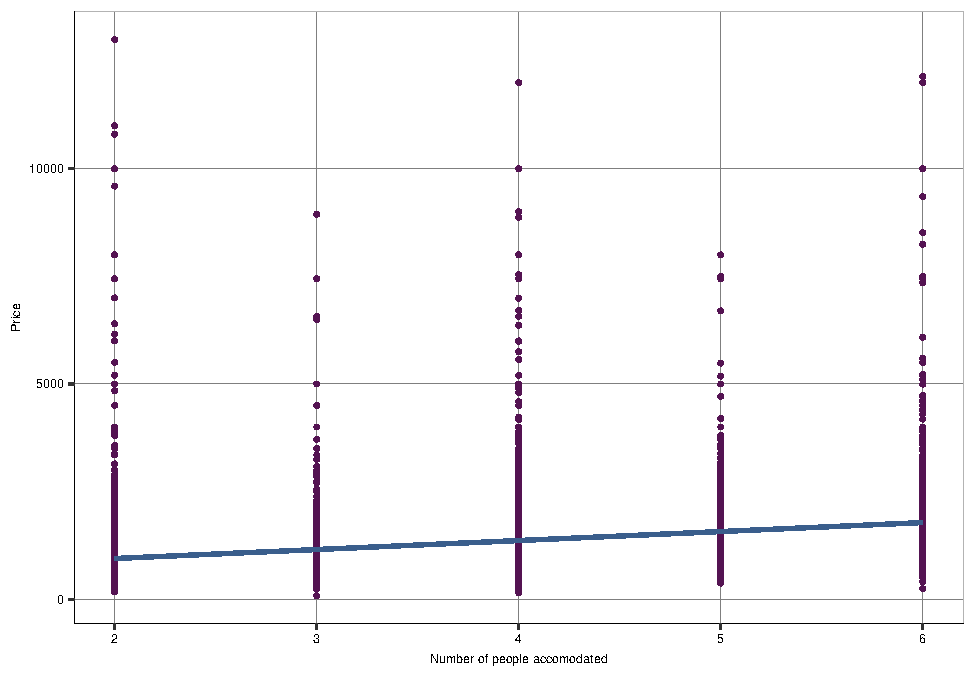
\includegraphics{A1_files/figure-latex/unnamed-chunk-10-1.pdf}

\begin{Shaded}
\begin{Highlighting}[]
\CommentTok{\#2b) Native \& Foreign create binary!}

\FunctionTok{summary}\NormalTok{(}\FunctionTok{as.factor}\NormalTok{(data}\SpecialCharTok{$}\NormalTok{prcitshp)) }
\end{Highlighting}
\end{Shaded}

\begin{verbatim}
##         Foreign Born, Not a US Citizen Foreign Born, US Cit By Naturalization 
##                                     52                                    105 
##    Native, Born Abroad Of US Parent(s) Native, Born in PR or US Outlying Area 
##                                     31                                      8 
##                     Native, Born In US 
##                                   3358
\end{verbatim}

\begin{Shaded}
\begin{Highlighting}[]
\CommentTok{\# graph: earnings distribution Citizenship status (boxplot)}

\NormalTok{boxplot\_native }\OtherTok{\textless{}{-}} \FunctionTok{ggplot}\NormalTok{(data, }\FunctionTok{aes}\NormalTok{(}\AttributeTok{x =}\NormalTok{ prcitshp, }\AttributeTok{y =}\NormalTok{ earnh)) }\SpecialCharTok{+}
  \FunctionTok{stat\_boxplot}\NormalTok{(}\FunctionTok{aes}\NormalTok{(}\AttributeTok{group =}\NormalTok{ prcitshp), }\AttributeTok{geom =} \StringTok{"errorbar"}\NormalTok{, }\AttributeTok{width =} \FloatTok{0.3}\NormalTok{,}
               \AttributeTok{color =} \FunctionTok{c}\NormalTok{(color[}\DecValTok{5}\NormalTok{],color[}\DecValTok{4}\NormalTok{],color[}\DecValTok{3}\NormalTok{],color[}\DecValTok{2}\NormalTok{],color[}\DecValTok{1}\NormalTok{]), }\AttributeTok{size =} \FloatTok{0.5}\NormalTok{, }\AttributeTok{na.rm=}\NormalTok{T)}\SpecialCharTok{+}
  \FunctionTok{geom\_boxplot}\NormalTok{(}\FunctionTok{aes}\NormalTok{(}\AttributeTok{group =}\NormalTok{ prcitshp),}
               \AttributeTok{color =} \FunctionTok{c}\NormalTok{(color[}\DecValTok{5}\NormalTok{],color[}\DecValTok{4}\NormalTok{],color[}\DecValTok{3}\NormalTok{],color[}\DecValTok{2}\NormalTok{],color[}\DecValTok{1}\NormalTok{]), }\AttributeTok{fill =} \FunctionTok{c}\NormalTok{(color[}\DecValTok{5}\NormalTok{],color[}\DecValTok{4}\NormalTok{],color[}\DecValTok{3}\NormalTok{],color[}\DecValTok{2}\NormalTok{],color[}\DecValTok{1}\NormalTok{]),}
               \AttributeTok{size =} \FloatTok{0.5}\NormalTok{, }\AttributeTok{width =} \FloatTok{0.6}\NormalTok{, }\AttributeTok{alpha =} \FloatTok{0.3}\NormalTok{, }\AttributeTok{na.rm=}\NormalTok{T, }\AttributeTok{outlier.shape =} \ConstantTok{NA}\NormalTok{) }\SpecialCharTok{+}
  \FunctionTok{labs}\NormalTok{(}\AttributeTok{x =} \StringTok{"Citizenship status"}\NormalTok{,}\AttributeTok{y =} \StringTok{"Earnings per hour"}\NormalTok{)}\SpecialCharTok{+}
  \FunctionTok{theme\_bg}\NormalTok{()}\SpecialCharTok{+}
    \FunctionTok{scale\_x\_discrete}\NormalTok{(}\AttributeTok{labels =} \FunctionTok{label\_wrap}\NormalTok{(}\DecValTok{10}\NormalTok{)) }

\NormalTok{boxplot\_native}
\end{Highlighting}
\end{Shaded}

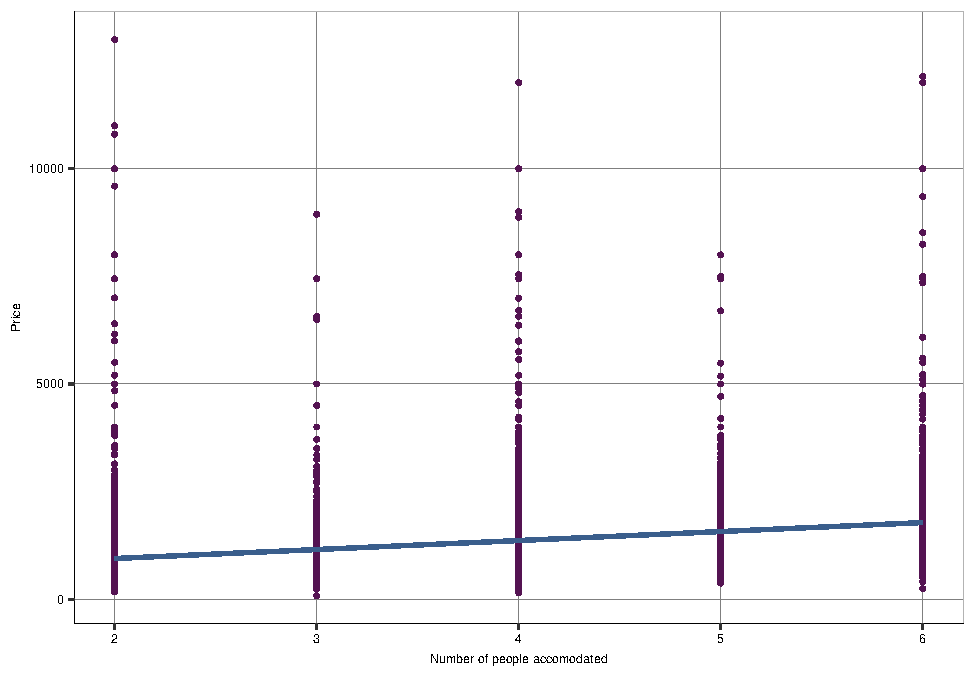
\includegraphics{A1_files/figure-latex/unnamed-chunk-11-1.pdf}

\begin{Shaded}
\begin{Highlighting}[]
\CommentTok{\# Native binary }

\NormalTok{data }\OtherTok{\textless{}{-}}\NormalTok{ data }\SpecialCharTok{\%\textgreater{}\%} \FunctionTok{mutate}\NormalTok{(}\AttributeTok{native =} \FunctionTok{ifelse}\NormalTok{(prcitshp}\SpecialCharTok{==}\StringTok{"Native, Born Abroad Of US Parent(s)"}\NormalTok{,}\DecValTok{1}\NormalTok{,}\FunctionTok{ifelse}\NormalTok{(prcitshp}\SpecialCharTok{==}\StringTok{"Native, Born in PR or US Outlying Area"}\NormalTok{,}\DecValTok{1}\NormalTok{,}\FunctionTok{ifelse}\NormalTok{(prcitshp}\SpecialCharTok{==}\StringTok{"Native, Born In US"}\NormalTok{,}\DecValTok{1}\NormalTok{,}\DecValTok{0}\NormalTok{))))}

\FunctionTok{summary}\NormalTok{(}\FunctionTok{as.factor}\NormalTok{(data}\SpecialCharTok{$}\NormalTok{native)) }
\end{Highlighting}
\end{Shaded}

\begin{verbatim}
##    0    1 
##  157 3397
\end{verbatim}

\begin{Shaded}
\begin{Highlighting}[]
\CommentTok{\# graph: earnings distribution native \& foreign (boxplot)}

\NormalTok{boxplot\_native2 }\OtherTok{\textless{}{-}} \FunctionTok{ggplot}\NormalTok{(data, }\FunctionTok{aes}\NormalTok{(}\AttributeTok{x =}\NormalTok{ native, }\AttributeTok{y =}\NormalTok{ earnh)) }\SpecialCharTok{+}
  \FunctionTok{stat\_boxplot}\NormalTok{(}\FunctionTok{aes}\NormalTok{(}\AttributeTok{group =}\NormalTok{ native), }\AttributeTok{geom =} \StringTok{"errorbar"}\NormalTok{, }\AttributeTok{width =} \FloatTok{0.3}\NormalTok{,}
               \AttributeTok{color =} \FunctionTok{c}\NormalTok{(color[}\DecValTok{2}\NormalTok{],color[}\DecValTok{1}\NormalTok{]), }\AttributeTok{size =} \FloatTok{0.5}\NormalTok{, }\AttributeTok{na.rm=}\NormalTok{T)}\SpecialCharTok{+}
  \FunctionTok{geom\_boxplot}\NormalTok{(}\FunctionTok{aes}\NormalTok{(}\AttributeTok{group =}\NormalTok{ native),}
               \AttributeTok{color =} \FunctionTok{c}\NormalTok{(color[}\DecValTok{2}\NormalTok{],color[}\DecValTok{1}\NormalTok{]), }\AttributeTok{fill =} \FunctionTok{c}\NormalTok{(color[}\DecValTok{2}\NormalTok{],color[}\DecValTok{1}\NormalTok{]),}
               \AttributeTok{size =} \FloatTok{0.5}\NormalTok{, }\AttributeTok{width =} \FloatTok{0.6}\NormalTok{, }\AttributeTok{alpha =} \FloatTok{0.3}\NormalTok{, }\AttributeTok{na.rm=}\NormalTok{T, }\AttributeTok{outlier.shape =} \ConstantTok{NA}\NormalTok{) }\SpecialCharTok{+}
  \FunctionTok{labs}\NormalTok{(}\AttributeTok{x =} \StringTok{"Citizenship status (0 = foreign, 1= native)"}\NormalTok{,}\AttributeTok{y =} \StringTok{"Earnings per hour"}\NormalTok{)}\SpecialCharTok{+}
  \FunctionTok{theme\_bg}\NormalTok{()}

\NormalTok{boxplot\_native2}
\end{Highlighting}
\end{Shaded}

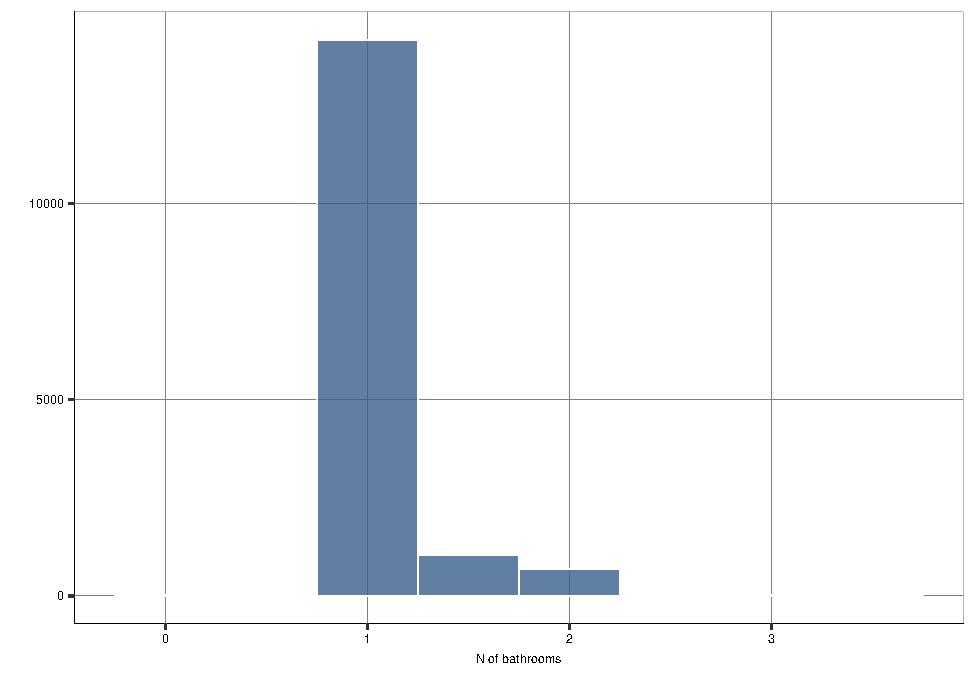
\includegraphics{A1_files/figure-latex/unnamed-chunk-11-2.pdf}

\begin{Shaded}
\begin{Highlighting}[]
\NormalTok{data }\SpecialCharTok{\%\textgreater{}\%}\NormalTok{ dplyr}\SpecialCharTok{::}\FunctionTok{select}\NormalTok{(earnh,native) }\SpecialCharTok{\%\textgreater{}\%} \FunctionTok{filter}\NormalTok{(native}\SpecialCharTok{==}\DecValTok{1}\NormalTok{) }\SpecialCharTok{\%\textgreater{}\%} \FunctionTok{summary}\NormalTok{()}
\end{Highlighting}
\end{Shaded}

\begin{verbatim}
##      earnh            native 
##  Min.   : 1.603   Min.   :1  
##  1st Qu.:16.827   1st Qu.:1  
##  Median :23.026   Median :1  
##  Mean   :24.666   Mean   :1  
##  3rd Qu.:30.288   3rd Qu.:1  
##  Max.   :64.900   Max.   :1
\end{verbatim}

\begin{Shaded}
\begin{Highlighting}[]
\NormalTok{data }\SpecialCharTok{\%\textgreater{}\%}\NormalTok{ dplyr}\SpecialCharTok{::}\FunctionTok{select}\NormalTok{(earnh,native) }\SpecialCharTok{\%\textgreater{}\%} \FunctionTok{filter}\NormalTok{(native}\SpecialCharTok{==}\DecValTok{0}\NormalTok{) }\SpecialCharTok{\%\textgreater{}\%} \FunctionTok{summary}\NormalTok{()}
\end{Highlighting}
\end{Shaded}

\begin{verbatim}
##      earnh           native 
##  Min.   : 3.26   Min.   :0  
##  1st Qu.:16.50   1st Qu.:0  
##  Median :23.08   Median :0  
##  Mean   :24.91   Mean   :0  
##  3rd Qu.:31.25   3rd Qu.:0  
##  Max.   :62.50   Max.   :0
\end{verbatim}

\begin{Shaded}
\begin{Highlighting}[]
\CommentTok{\#2c) \# class of worker: private / gov. Create binary! }

\FunctionTok{summary}\NormalTok{(}\FunctionTok{as.factor}\NormalTok{(data}\SpecialCharTok{$}\NormalTok{class)) }
\end{Highlighting}
\end{Shaded}

\begin{verbatim}
## Government - Federal   Government - Local   Government - State 
##                   20                 2148                  677 
##  Private, For Profit   Private, Nonprofit 
##                  438                  271
\end{verbatim}

\begin{Shaded}
\begin{Highlighting}[]
\NormalTok{boxplot\_class2 }\OtherTok{\textless{}{-}} \FunctionTok{ggplot}\NormalTok{(data, }\FunctionTok{aes}\NormalTok{(}\AttributeTok{x =}\NormalTok{ class, }\AttributeTok{y =}\NormalTok{ earnh)) }\SpecialCharTok{+}
  \FunctionTok{stat\_boxplot}\NormalTok{(}\FunctionTok{aes}\NormalTok{(}\AttributeTok{group =}\NormalTok{ class), }\AttributeTok{geom =} \StringTok{"errorbar"}\NormalTok{, }\AttributeTok{width =} \FloatTok{0.3}\NormalTok{,}
               \AttributeTok{color =} \FunctionTok{c}\NormalTok{(color[}\DecValTok{5}\NormalTok{],color[}\DecValTok{4}\NormalTok{],color[}\DecValTok{3}\NormalTok{],color[}\DecValTok{2}\NormalTok{],color[}\DecValTok{1}\NormalTok{]), }\AttributeTok{size =} \FloatTok{0.5}\NormalTok{, }\AttributeTok{na.rm=}\NormalTok{T)}\SpecialCharTok{+}
  \FunctionTok{geom\_boxplot}\NormalTok{(}\FunctionTok{aes}\NormalTok{(}\AttributeTok{group =}\NormalTok{ class),}
               \AttributeTok{color =} \FunctionTok{c}\NormalTok{(color[}\DecValTok{5}\NormalTok{],color[}\DecValTok{4}\NormalTok{],color[}\DecValTok{3}\NormalTok{],color[}\DecValTok{2}\NormalTok{],color[}\DecValTok{1}\NormalTok{]), }\AttributeTok{fill =} \FunctionTok{c}\NormalTok{(color[}\DecValTok{5}\NormalTok{],color[}\DecValTok{4}\NormalTok{],color[}\DecValTok{3}\NormalTok{],color[}\DecValTok{2}\NormalTok{],color[}\DecValTok{1}\NormalTok{]),}
               \AttributeTok{size =} \FloatTok{0.5}\NormalTok{, }\AttributeTok{width =} \FloatTok{0.6}\NormalTok{, }\AttributeTok{alpha =} \FloatTok{0.3}\NormalTok{, }\AttributeTok{na.rm=}\NormalTok{T, }\AttributeTok{outlier.shape =} \ConstantTok{NA}\NormalTok{) }\SpecialCharTok{+}
  \FunctionTok{labs}\NormalTok{(}\AttributeTok{x =} \StringTok{"Class of worker"}\NormalTok{,}\AttributeTok{y =} \StringTok{"Earnings per hour"}\NormalTok{)}\SpecialCharTok{+}
  \FunctionTok{theme\_bg}\NormalTok{()}

\NormalTok{boxplot\_class2}
\end{Highlighting}
\end{Shaded}

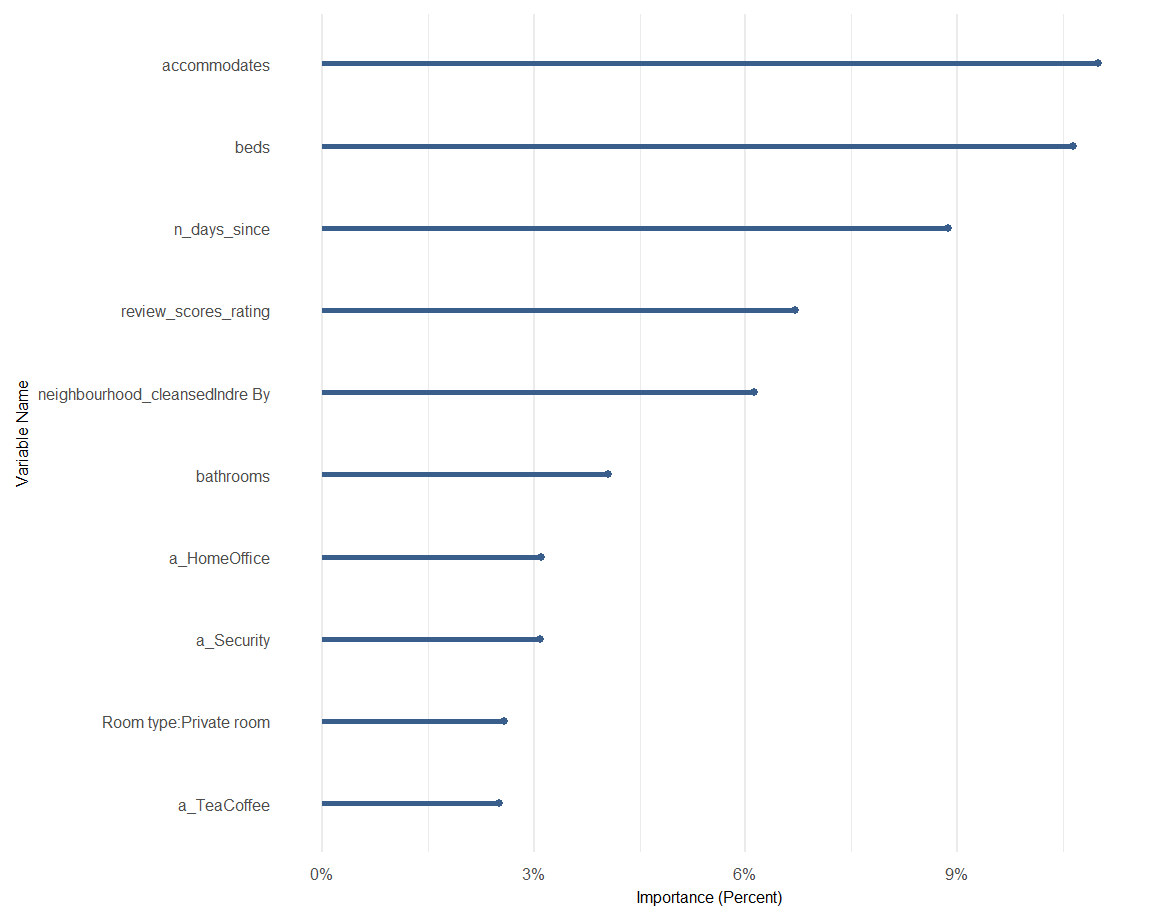
\includegraphics{A1_files/figure-latex/unnamed-chunk-12-1.pdf}

\begin{Shaded}
\begin{Highlighting}[]
\CommentTok{\# change to binary }

\NormalTok{data }\OtherTok{\textless{}{-}}\NormalTok{ data }\SpecialCharTok{\%\textgreater{}\%} \FunctionTok{mutate}\NormalTok{(}\AttributeTok{private =} \FunctionTok{ifelse}\NormalTok{(class }\SpecialCharTok{==} \StringTok{"Private, For Profit"}\NormalTok{,}\DecValTok{1}\NormalTok{,}\FunctionTok{ifelse}\NormalTok{(class }\SpecialCharTok{==} \StringTok{"Private, Nonprofit"}\NormalTok{,}\DecValTok{1}\NormalTok{,}\DecValTok{0}\NormalTok{)))}

\FunctionTok{summary}\NormalTok{(}\FunctionTok{as.factor}\NormalTok{(data}\SpecialCharTok{$}\NormalTok{private)) }
\end{Highlighting}
\end{Shaded}

\begin{verbatim}
##    0    1 
## 2845  709
\end{verbatim}

\begin{Shaded}
\begin{Highlighting}[]
\NormalTok{boxplot\_class }\OtherTok{\textless{}{-}} \FunctionTok{ggplot}\NormalTok{(data, }\FunctionTok{aes}\NormalTok{(}\AttributeTok{x =}\NormalTok{ private, }\AttributeTok{y =}\NormalTok{ earnh)) }\SpecialCharTok{+}
  \FunctionTok{stat\_boxplot}\NormalTok{(}\FunctionTok{aes}\NormalTok{(}\AttributeTok{group =}\NormalTok{ private), }\AttributeTok{geom =} \StringTok{"errorbar"}\NormalTok{, }\AttributeTok{width =} \FloatTok{0.3}\NormalTok{,}
               \AttributeTok{color =} \FunctionTok{c}\NormalTok{(color[}\DecValTok{2}\NormalTok{],color[}\DecValTok{1}\NormalTok{]), }\AttributeTok{size =} \FloatTok{0.5}\NormalTok{, }\AttributeTok{na.rm=}\NormalTok{T)}\SpecialCharTok{+}
  \FunctionTok{geom\_boxplot}\NormalTok{(}\FunctionTok{aes}\NormalTok{(}\AttributeTok{group =}\NormalTok{ private),}
               \AttributeTok{color =} \FunctionTok{c}\NormalTok{(color[}\DecValTok{2}\NormalTok{],color[}\DecValTok{1}\NormalTok{]), }\AttributeTok{fill =} \FunctionTok{c}\NormalTok{(color[}\DecValTok{2}\NormalTok{],color[}\DecValTok{1}\NormalTok{]),}
               \AttributeTok{size =} \FloatTok{0.5}\NormalTok{, }\AttributeTok{width =} \FloatTok{0.6}\NormalTok{, }\AttributeTok{alpha =} \FloatTok{0.3}\NormalTok{, }\AttributeTok{na.rm=}\NormalTok{T, }\AttributeTok{outlier.shape =} \ConstantTok{NA}\NormalTok{) }\SpecialCharTok{+}
  \FunctionTok{labs}\NormalTok{(}\AttributeTok{x =} \StringTok{"Class of worker (0 = government, 1 = private)"}\NormalTok{,}\AttributeTok{y =} \StringTok{"Earnings per hour"}\NormalTok{)}\SpecialCharTok{+}
  \FunctionTok{theme\_bg}\NormalTok{()}

\NormalTok{boxplot\_class}
\end{Highlighting}
\end{Shaded}

\includegraphics{A1_files/figure-latex/unnamed-chunk-12-2.pdf}

\begin{Shaded}
\begin{Highlighting}[]
\CommentTok{\# add graph: earnings distribution private \& gov (boxplot)}
\end{Highlighting}
\end{Shaded}

\begin{Shaded}
\begin{Highlighting}[]
\CommentTok{\#2) race binary as: white and other.}

\FunctionTok{summary}\NormalTok{(}\FunctionTok{as.factor}\NormalTok{(data}\SpecialCharTok{$}\NormalTok{race)) }
\end{Highlighting}
\end{Shaded}

\begin{verbatim}
##    1    2    3    4    5    6    7    8    9   10   11   13   15   16   21 
## 3123  288   19   73   13    7    6    6    5    1    1    1    3    4    4
\end{verbatim}

\begin{Shaded}
\begin{Highlighting}[]
\NormalTok{data }\OtherTok{\textless{}{-}}\NormalTok{ data }\SpecialCharTok{\%\textgreater{}\%} \FunctionTok{mutate}\NormalTok{(}\AttributeTok{white =} \FunctionTok{ifelse}\NormalTok{(race }\SpecialCharTok{==} \DecValTok{1}\NormalTok{ ,}\DecValTok{1}\NormalTok{,}\DecValTok{0}\NormalTok{))}

\FunctionTok{summary}\NormalTok{(}\FunctionTok{as.factor}\NormalTok{(data}\SpecialCharTok{$}\NormalTok{white))}
\end{Highlighting}
\end{Shaded}

\begin{verbatim}
##    0    1 
##  431 3123
\end{verbatim}

\begin{Shaded}
\begin{Highlighting}[]
\NormalTok{boxplot\_race }\OtherTok{\textless{}{-}} \FunctionTok{ggplot}\NormalTok{(data, }\FunctionTok{aes}\NormalTok{(}\AttributeTok{x =}\NormalTok{ white, }\AttributeTok{y =}\NormalTok{ earnh)) }\SpecialCharTok{+}
  \FunctionTok{stat\_boxplot}\NormalTok{(}\FunctionTok{aes}\NormalTok{(}\AttributeTok{group =}\NormalTok{ white), }\AttributeTok{geom =} \StringTok{"errorbar"}\NormalTok{, }\AttributeTok{width =} \FloatTok{0.3}\NormalTok{,}
               \AttributeTok{color =} \FunctionTok{c}\NormalTok{(color[}\DecValTok{2}\NormalTok{],color[}\DecValTok{1}\NormalTok{]), }\AttributeTok{size =} \FloatTok{0.5}\NormalTok{, }\AttributeTok{na.rm=}\NormalTok{T)}\SpecialCharTok{+}
  \FunctionTok{geom\_boxplot}\NormalTok{(}\FunctionTok{aes}\NormalTok{(}\AttributeTok{group =}\NormalTok{ white),}
               \AttributeTok{color =} \FunctionTok{c}\NormalTok{(color[}\DecValTok{2}\NormalTok{],color[}\DecValTok{1}\NormalTok{]), }\AttributeTok{fill =} \FunctionTok{c}\NormalTok{(color[}\DecValTok{2}\NormalTok{],color[}\DecValTok{1}\NormalTok{]),}
               \AttributeTok{size =} \FloatTok{0.5}\NormalTok{, }\AttributeTok{width =} \FloatTok{0.6}\NormalTok{, }\AttributeTok{alpha =} \FloatTok{0.3}\NormalTok{, }\AttributeTok{na.rm=}\NormalTok{T, }\AttributeTok{outlier.shape =} \ConstantTok{NA}\NormalTok{) }\SpecialCharTok{+}
  \FunctionTok{labs}\NormalTok{(}\AttributeTok{x =} \StringTok{"Race (White = 1, Else = 0)"}\NormalTok{,}\AttributeTok{y =} \StringTok{"Earnings per hour"}\NormalTok{)}\SpecialCharTok{+}
  \FunctionTok{theme\_bg}\NormalTok{()}

\NormalTok{boxplot\_race}
\end{Highlighting}
\end{Shaded}

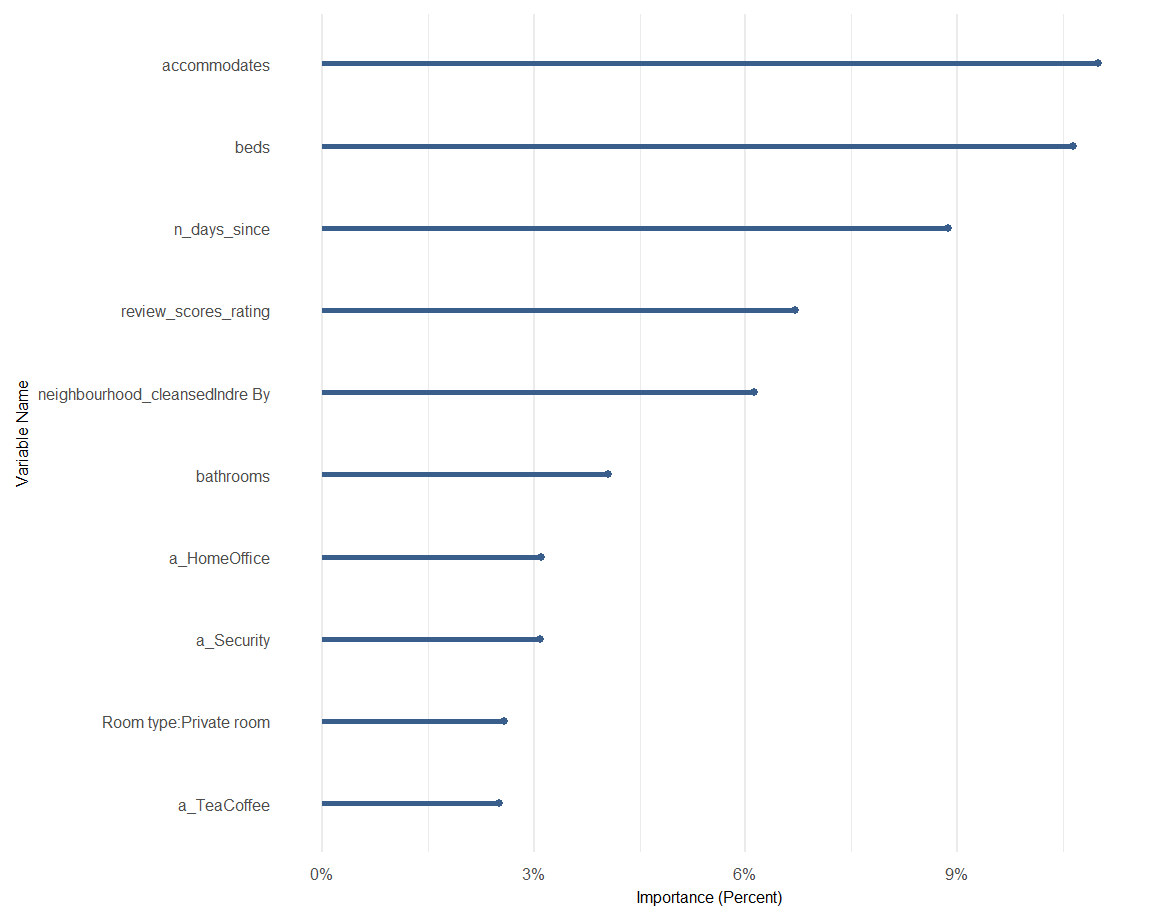
\includegraphics{A1_files/figure-latex/unnamed-chunk-13-1.pdf}

\begin{Shaded}
\begin{Highlighting}[]
\CommentTok{\# 2d) Education level. Create binaries.  }

\FunctionTok{summary}\NormalTok{(}\FunctionTok{as.factor}\NormalTok{(data}\SpecialCharTok{$}\NormalTok{grade92)) }
\end{Highlighting}
\end{Shaded}

\begin{verbatim}
##   38   39   40   41   42   43   44   45   46 
##    5   72  103   31   66 1521 1671   46   39
\end{verbatim}

\begin{Shaded}
\begin{Highlighting}[]
\CommentTok{\#graph: earnings distribution education levels }


\CommentTok{\#38 12th grade NO DIPLOMA}
\CommentTok{\#39 High school graduate, diploma or GED START }
\CommentTok{\#40 Some college but no degree }
\CommentTok{\#41 Associate degree {-}{-} occupational/vocational }
\CommentTok{\#42 Associate degree {-}{-} occupational/vocational }
\CommentTok{\#43 Bachelor\textquotesingle{}s degree (e.g. BA,AB,BS) }
\CommentTok{\#44 Master\textquotesingle{}s degree (e.g. MA,MS,MEng,Med,MSW,MBA) }
\CommentTok{\#45 Professional school deg. (e.g. MD,DDS,DVM,LLB,JD)}
\CommentTok{\#46 Doctorate degree (e.g. PhD, EdD) }

\NormalTok{boxplot\_grade92 }\OtherTok{\textless{}{-}} \FunctionTok{ggplot}\NormalTok{(data, }\FunctionTok{aes}\NormalTok{(}\AttributeTok{x =}\NormalTok{ grade92, }\AttributeTok{y =}\NormalTok{ earnh)) }\SpecialCharTok{+}
  \FunctionTok{stat\_boxplot}\NormalTok{(}\FunctionTok{aes}\NormalTok{(}\AttributeTok{group =}\NormalTok{ grade92), }\AttributeTok{geom =} \StringTok{"errorbar"}\NormalTok{, }\AttributeTok{width =} \FloatTok{0.3}\NormalTok{,}
               \AttributeTok{color =} \FunctionTok{c}\NormalTok{(color[}\DecValTok{1}\NormalTok{],color[}\DecValTok{2}\NormalTok{],color[}\DecValTok{3}\NormalTok{],color[}\DecValTok{4}\NormalTok{],color[}\DecValTok{5}\NormalTok{],color[}\DecValTok{4}\NormalTok{],color[}\DecValTok{3}\NormalTok{],color[}\DecValTok{2}\NormalTok{],color[}\DecValTok{1}\NormalTok{]), }\AttributeTok{size =} \FloatTok{0.5}\NormalTok{, }\AttributeTok{na.rm=}\NormalTok{T)}\SpecialCharTok{+}
  \FunctionTok{geom\_boxplot}\NormalTok{(}\FunctionTok{aes}\NormalTok{(}\AttributeTok{group =}\NormalTok{ grade92),}
               \AttributeTok{color =} \FunctionTok{c}\NormalTok{(color[}\DecValTok{1}\NormalTok{],color[}\DecValTok{2}\NormalTok{],color[}\DecValTok{3}\NormalTok{],color[}\DecValTok{4}\NormalTok{],color[}\DecValTok{5}\NormalTok{],color[}\DecValTok{4}\NormalTok{],color[}\DecValTok{3}\NormalTok{],color[}\DecValTok{2}\NormalTok{],color[}\DecValTok{1}\NormalTok{]), }\AttributeTok{fill =} \FunctionTok{c}\NormalTok{(color[}\DecValTok{1}\NormalTok{],color[}\DecValTok{2}\NormalTok{],color[}\DecValTok{3}\NormalTok{],color[}\DecValTok{4}\NormalTok{],color[}\DecValTok{5}\NormalTok{],color[}\DecValTok{4}\NormalTok{],color[}\DecValTok{3}\NormalTok{],color[}\DecValTok{2}\NormalTok{],color[}\DecValTok{1}\NormalTok{]),}
               \AttributeTok{size =} \FloatTok{0.5}\NormalTok{, }\AttributeTok{width =} \FloatTok{0.6}\NormalTok{, }\AttributeTok{alpha =} \FloatTok{0.3}\NormalTok{, }\AttributeTok{na.rm=}\NormalTok{T, }\AttributeTok{outlier.shape =} \ConstantTok{NA}\NormalTok{) }\SpecialCharTok{+}
  \FunctionTok{labs}\NormalTok{(}\AttributeTok{x =} \StringTok{"Education level"}\NormalTok{,}\AttributeTok{y =} \StringTok{"Earnings per hour"}\NormalTok{)}\SpecialCharTok{+}
  \FunctionTok{scale\_x\_continuous}\NormalTok{(}\AttributeTok{limits =}\FunctionTok{c}\NormalTok{(}\DecValTok{37}\NormalTok{,}\DecValTok{47}\NormalTok{), }\AttributeTok{breaks =} \FunctionTok{seq}\NormalTok{(}\DecValTok{38}\NormalTok{,}\DecValTok{46}\NormalTok{, }\DecValTok{1}\NormalTok{),}\AttributeTok{label =} \FunctionTok{c}\NormalTok{(}\StringTok{"12th grade NO DIPLOMA"}\NormalTok{, }\StringTok{"High school graduate, diploma or GED START"}\NormalTok{, }\StringTok{"Some college but no degree"}\NormalTok{,}\StringTok{"Associate degree {-}{-} occupational/vocational"}\NormalTok{,}\StringTok{"Associate degree {-}{-} academic"}\NormalTok{, }\StringTok{"Bachelor\textquotesingle{}s degree"}\NormalTok{, }\StringTok{"Master\textquotesingle{}s degree"}\NormalTok{, }\StringTok{"Professional school deg."}\NormalTok{, }\StringTok{"Doctorate degree"}\NormalTok{))}\SpecialCharTok{+}
  \FunctionTok{theme\_bg}\NormalTok{() }\SpecialCharTok{+}
  \FunctionTok{coord\_flip}\NormalTok{()}

\NormalTok{boxplot\_grade92}
\end{Highlighting}
\end{Shaded}

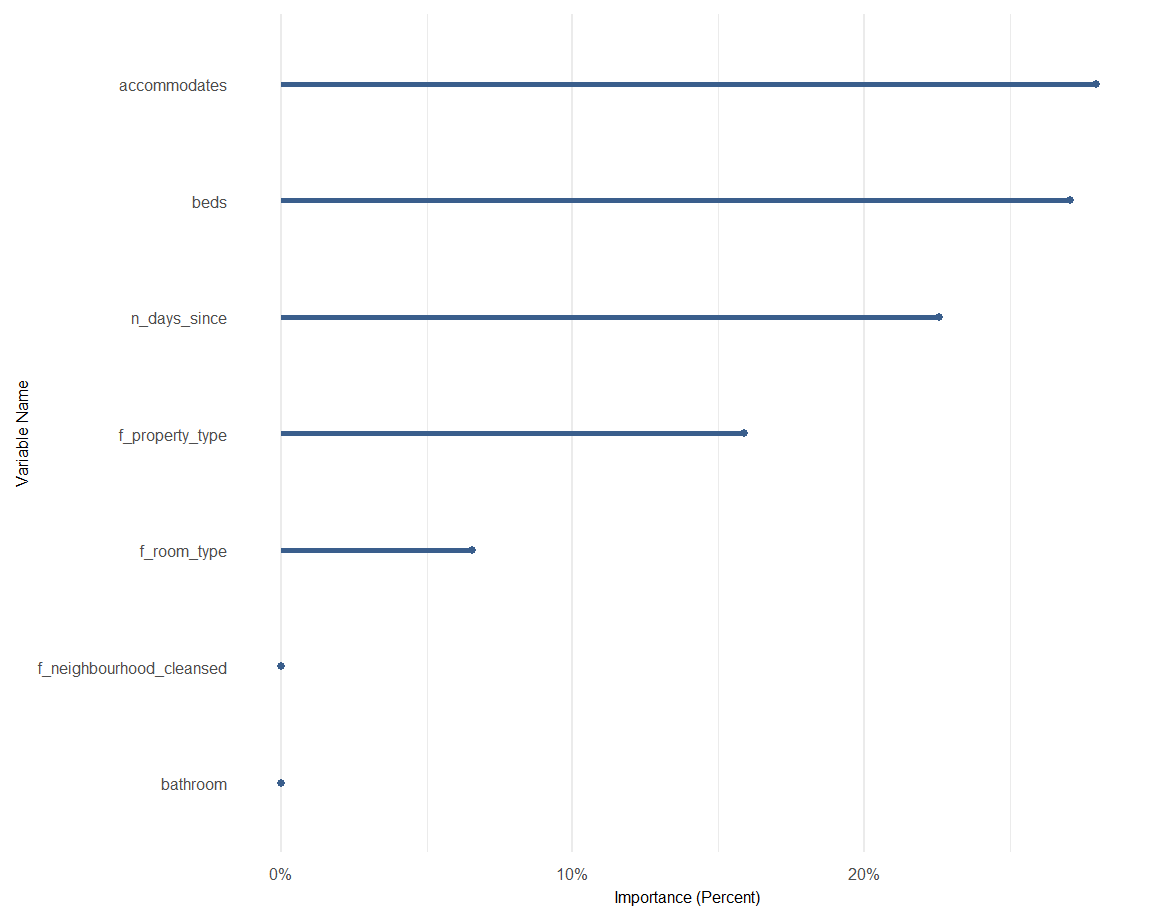
\includegraphics{A1_files/figure-latex/unnamed-chunk-14-1.pdf}

\begin{Shaded}
\begin{Highlighting}[]
\NormalTok{data  }\OtherTok{\textless{}{-}}\NormalTok{ data }\SpecialCharTok{\%\textgreater{}\%} \FunctionTok{mutate}\NormalTok{(}\AttributeTok{edu\_HighS =} \FunctionTok{as.numeric}\NormalTok{(grade92}\SpecialCharTok{==}\DecValTok{38}\NormalTok{),}
                        \AttributeTok{edu\_BA =} \FunctionTok{as.numeric}\NormalTok{(grade92}\SpecialCharTok{==}\DecValTok{43}\NormalTok{),}
                        \AttributeTok{edu\_MA=}\FunctionTok{as.numeric}\NormalTok{(grade92}\SpecialCharTok{==}\DecValTok{44}\NormalTok{),}
                        \AttributeTok{edu\_Prof =} \FunctionTok{as.numeric}\NormalTok{(grade92}\SpecialCharTok{==}\DecValTok{45}\NormalTok{),}
                        \AttributeTok{edu\_PhD =} \FunctionTok{as.numeric}\NormalTok{(grade92}\SpecialCharTok{==}\DecValTok{46}\NormalTok{))}
\end{Highlighting}
\end{Shaded}

\begin{Shaded}
\begin{Highlighting}[]
\CommentTok{\#2e) UNION Do as 1,0 }
\FunctionTok{summary}\NormalTok{(}\FunctionTok{as.factor}\NormalTok{(data}\SpecialCharTok{$}\NormalTok{unionmme))}
\end{Highlighting}
\end{Shaded}

\begin{verbatim}
##   No  Yes 
## 1727 1827
\end{verbatim}

\begin{Shaded}
\begin{Highlighting}[]
\FunctionTok{summary}\NormalTok{(}\FunctionTok{as.factor}\NormalTok{(data}\SpecialCharTok{$}\NormalTok{unioncov))}
\end{Highlighting}
\end{Shaded}

\begin{verbatim}
##      No     Yes Missing 
##    1565     162    1827
\end{verbatim}

\begin{Shaded}
\begin{Highlighting}[]
\NormalTok{data }\OtherTok{\textless{}{-}}\NormalTok{ data }\SpecialCharTok{\%\textgreater{}\%} \FunctionTok{mutate}\NormalTok{(}\AttributeTok{union =} \FunctionTok{as.numeric}\NormalTok{(unionmme}\SpecialCharTok{==}\StringTok{"Yes"} \SpecialCharTok{|}\NormalTok{ unioncov}\SpecialCharTok{==}\StringTok{"Yes"}\NormalTok{))}

\NormalTok{boxplot\_union }\OtherTok{\textless{}{-}} \FunctionTok{ggplot}\NormalTok{(data, }\FunctionTok{aes}\NormalTok{(}\AttributeTok{x =}\NormalTok{ union, }\AttributeTok{y =}\NormalTok{ earnh)) }\SpecialCharTok{+}
  \FunctionTok{stat\_boxplot}\NormalTok{(}\FunctionTok{aes}\NormalTok{(}\AttributeTok{group =}\NormalTok{ union), }\AttributeTok{geom =} \StringTok{"errorbar"}\NormalTok{, }\AttributeTok{width =} \FloatTok{0.3}\NormalTok{,}
               \AttributeTok{color =} \FunctionTok{c}\NormalTok{(color[}\DecValTok{2}\NormalTok{],color[}\DecValTok{1}\NormalTok{]), }\AttributeTok{size =} \FloatTok{0.5}\NormalTok{, }\AttributeTok{na.rm=}\NormalTok{T)}\SpecialCharTok{+}
  \FunctionTok{geom\_boxplot}\NormalTok{(}\FunctionTok{aes}\NormalTok{(}\AttributeTok{group =}\NormalTok{ union),}
               \AttributeTok{color =} \FunctionTok{c}\NormalTok{(color[}\DecValTok{2}\NormalTok{],color[}\DecValTok{1}\NormalTok{]), }\AttributeTok{fill =} \FunctionTok{c}\NormalTok{(color[}\DecValTok{2}\NormalTok{],color[}\DecValTok{1}\NormalTok{]),}
               \AttributeTok{size =} \FloatTok{0.5}\NormalTok{, }\AttributeTok{width =} \FloatTok{0.6}\NormalTok{, }\AttributeTok{alpha =} \FloatTok{0.3}\NormalTok{, }\AttributeTok{na.rm=}\NormalTok{T, }\AttributeTok{outlier.shape =} \ConstantTok{NA}\NormalTok{) }\SpecialCharTok{+}
  \FunctionTok{labs}\NormalTok{(}\AttributeTok{x =} \StringTok{"Union (0 = No, 1 = Yes)"}\NormalTok{,}\AttributeTok{y =} \StringTok{"Earnings per hour"}\NormalTok{)}\SpecialCharTok{+}
  \FunctionTok{theme\_bg}\NormalTok{()}

\NormalTok{boxplot\_union}
\end{Highlighting}
\end{Shaded}

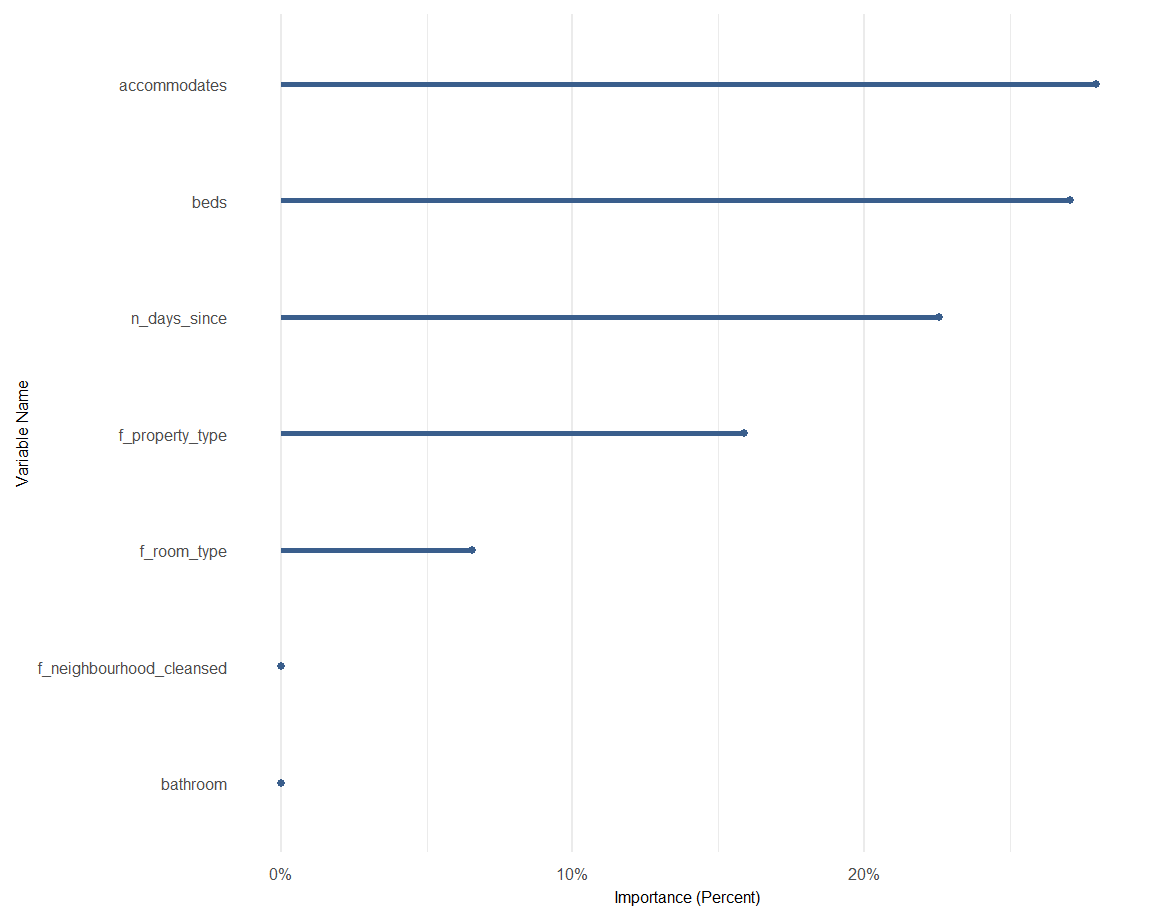
\includegraphics{A1_files/figure-latex/unnamed-chunk-15-1.pdf}

\hypertarget{furhter-demographics-family}{%
\section{Furhter demographics
(family)}\label{furhter-demographics-family}}

\begin{Shaded}
\begin{Highlighting}[]
\NormalTok{data }\OtherTok{\textless{}{-}}\NormalTok{ data }\SpecialCharTok{\%\textgreater{}\%} \FunctionTok{mutate}\NormalTok{(}\AttributeTok{married =} \FunctionTok{as.numeric}\NormalTok{(marital}\SpecialCharTok{==}\DecValTok{1} \SpecialCharTok{|}\NormalTok{ marital}\SpecialCharTok{==}\DecValTok{2}\NormalTok{),}
                      \AttributeTok{divorced =} \FunctionTok{as.numeric}\NormalTok{(marital}\SpecialCharTok{==}\DecValTok{3} \SpecialCharTok{|}\NormalTok{ marital}\SpecialCharTok{==}\DecValTok{5} \SpecialCharTok{|}\NormalTok{ marital}\SpecialCharTok{==}\DecValTok{6}\NormalTok{),}
                      \AttributeTok{wirowed =} \FunctionTok{as.numeric}\NormalTok{(marital}\SpecialCharTok{==}\DecValTok{4}\NormalTok{),}
                      \AttributeTok{nevermar =} \FunctionTok{as.numeric}\NormalTok{(marital}\SpecialCharTok{==}\DecValTok{7}\NormalTok{),}
                      \AttributeTok{child0 =} \FunctionTok{as.numeric}\NormalTok{(chldpres}\SpecialCharTok{==}\DecValTok{0}\NormalTok{),}
                      \AttributeTok{child1 =} \FunctionTok{as.numeric}\NormalTok{(chldpres}\SpecialCharTok{==}\DecValTok{1}\NormalTok{),}
                      \AttributeTok{child2 =} \FunctionTok{as.numeric}\NormalTok{(chldpres}\SpecialCharTok{==}\DecValTok{2}\NormalTok{),}
                      \AttributeTok{child3 =} \FunctionTok{as.numeric}\NormalTok{(chldpres}\SpecialCharTok{==}\DecValTok{3}\NormalTok{),}
                      \AttributeTok{child4plus =} \FunctionTok{as.numeric}\NormalTok{(chldpres}\SpecialCharTok{\textgreater{}=}\DecValTok{4}\NormalTok{))}
\CommentTok{\# no need for "ownchild" variable  }
\end{Highlighting}
\end{Shaded}

\begin{Shaded}
\begin{Highlighting}[]
\CommentTok{\# graph group by state? mean salary by state? }
\CommentTok{\# check frequency of teacher by state type}
\NormalTok{data }\SpecialCharTok{\%\textgreater{}\%}
  \FunctionTok{group\_by}\NormalTok{(stfips) }\SpecialCharTok{\%\textgreater{}\%}
\NormalTok{  dplyr}\SpecialCharTok{::}\FunctionTok{summarize}\NormalTok{(}\AttributeTok{frequency=}\FunctionTok{n}\NormalTok{()) }\SpecialCharTok{\%\textgreater{}\%}
  \FunctionTok{mutate}\NormalTok{(}\AttributeTok{percent =}\NormalTok{ frequency }\SpecialCharTok{/} \FunctionTok{sum}\NormalTok{(frequency)}\SpecialCharTok{*}\DecValTok{100}\NormalTok{)}
\end{Highlighting}
\end{Shaded}

\begin{verbatim}
## # A tibble: 51 x 3
##    stfips frequency percent
##    <chr>      <int>   <dbl>
##  1 AK            56   1.58 
##  2 AL            45   1.27 
##  3 AR            42   1.18 
##  4 AZ            33   0.929
##  5 CA           256   7.20 
##  6 CO            69   1.94 
##  7 CT            83   2.34 
##  8 DC            47   1.32 
##  9 DE            52   1.46 
## 10 FL           163   4.59 
## # i 41 more rows
\end{verbatim}

\begin{Shaded}
\begin{Highlighting}[]
\CommentTok{\# most teacher is CA,, FL, NY, TX}
\NormalTok{salary\_state }\OtherTok{\textless{}{-}} \FunctionTok{ggplot}\NormalTok{(data, }\FunctionTok{aes}\NormalTok{(}\FunctionTok{reorder}\NormalTok{(stfips, earnh, }\AttributeTok{FUN =}\NormalTok{ mean), earnh)) }\SpecialCharTok{+}
  \FunctionTok{geom\_bar}\NormalTok{(}\AttributeTok{position=}\StringTok{\textquotesingle{}dodge\textquotesingle{}}\NormalTok{, }\AttributeTok{stat=}\StringTok{\textquotesingle{}summary\textquotesingle{}}\NormalTok{, }\AttributeTok{fun=}\StringTok{\textquotesingle{}mean\textquotesingle{}}\NormalTok{,}\AttributeTok{binwidth =} \FloatTok{0.1}\NormalTok{, }\AttributeTok{fill =}\NormalTok{ color[}\DecValTok{1}\NormalTok{], }\AttributeTok{color =}\NormalTok{color.outline, }\AttributeTok{alpha =} \FloatTok{0.8}\NormalTok{, }\AttributeTok{size =} \FloatTok{0.25}\NormalTok{) }\SpecialCharTok{+}
   \FunctionTok{coord\_flip}\NormalTok{() }\SpecialCharTok{+}
  \FunctionTok{labs}\NormalTok{(}\AttributeTok{x =} \StringTok{"States"}\NormalTok{,}\AttributeTok{y =} \StringTok{"Earnings per hour (mean)"}\NormalTok{)}\SpecialCharTok{+}
  \FunctionTok{theme\_bg}\NormalTok{()}
\end{Highlighting}
\end{Shaded}

\begin{verbatim}
## Warning in geom_bar(position = "dodge", stat = "summary", fun = "mean", :
## Ignoring unknown parameters: `binwidth`
\end{verbatim}

\begin{Shaded}
\begin{Highlighting}[]
\NormalTok{salary\_state}
\end{Highlighting}
\end{Shaded}

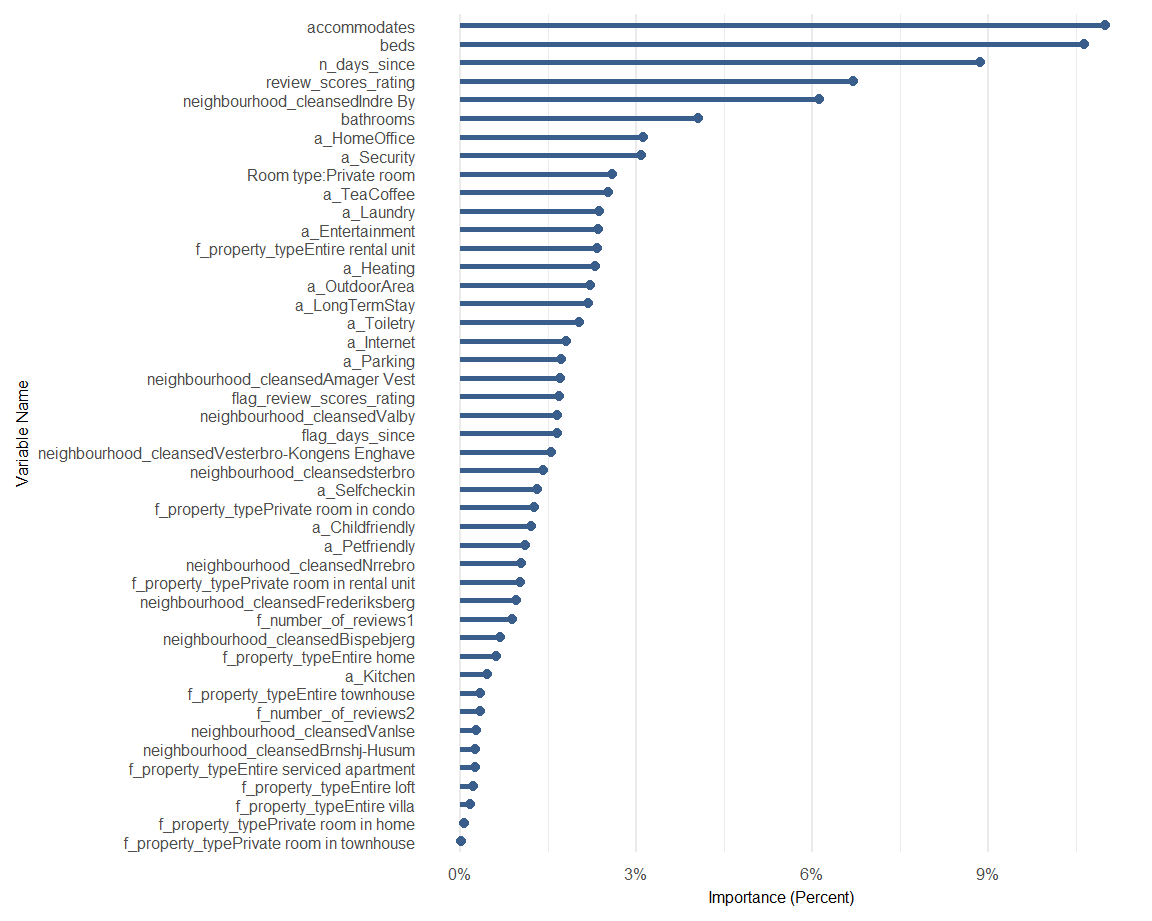
\includegraphics{A1_files/figure-latex/unnamed-chunk-17-1.pdf}

\begin{Shaded}
\begin{Highlighting}[]
\CommentTok{\# use as fixed effects {-} state }

\CommentTok{\# Continuous – nothing to do. Make sure it is stored as number}
\CommentTok{\#glimpse(data)}
\end{Highlighting}
\end{Shaded}

\hypertarget{functional-form-xs-plot-against-earning-per-hour}{%
\subsubsection{4) functional form X's (plot against earning per
hour)}\label{functional-form-xs-plot-against-earning-per-hour}}

\begin{Shaded}
\begin{Highlighting}[]
\CommentTok{\#4. Selecting functional form {-} log or sq of X\textquotesingle{}s}

\CommentTok{\# age sqaured }
\CommentTok{\#adding the square of the variable allows you to model more accurately the effect of age, which may have a non{-}linear relationship with the independent variable. For instance, the effect of age could be positive up until, say, the age of 50, and then negative thereafter.}

\CommentTok{\#Adding the age squared to age, allows you to model the effect a differing ages, rather than assuming the effect is linear for all ages.}

\NormalTok{data }\OtherTok{\textless{}{-}}\NormalTok{ data }\SpecialCharTok{\%\textgreater{}\%} \FunctionTok{mutate}\NormalTok{(}\AttributeTok{agesq=}\NormalTok{age}\SpecialCharTok{\^{}}\DecValTok{2}\NormalTok{,}
                        \AttributeTok{lnage =} \FunctionTok{log}\NormalTok{(age))}

\NormalTok{plot\_ageearnh }\OtherTok{\textless{}{-}} \FunctionTok{ggplot}\NormalTok{(}\AttributeTok{data =}\NormalTok{ data, }\FunctionTok{aes}\NormalTok{(}\AttributeTok{x=}\NormalTok{data}\SpecialCharTok{$}\NormalTok{age, }\AttributeTok{y=}\NormalTok{earnh)) }\SpecialCharTok{+}
  \FunctionTok{geom\_point}\NormalTok{( }\AttributeTok{color =}\NormalTok{ color[}\DecValTok{1}\NormalTok{], }\AttributeTok{size =} \DecValTok{1}\NormalTok{,  }\AttributeTok{shape =} \DecValTok{16}\NormalTok{, }\AttributeTok{alpha =} \FloatTok{0.8}\NormalTok{, }\AttributeTok{show.legend=}\NormalTok{F, }
              \AttributeTok{na.rm =} \ConstantTok{TRUE}\NormalTok{) }\SpecialCharTok{+} 
  \FunctionTok{geom\_smooth}\NormalTok{(}\AttributeTok{method=}\StringTok{"lm"}\NormalTok{, }\AttributeTok{se=}\NormalTok{F, }\AttributeTok{colour=}\NormalTok{color[}\DecValTok{4}\NormalTok{], }\AttributeTok{size=}\DecValTok{1}\NormalTok{, }\AttributeTok{span=}\FloatTok{0.9}\NormalTok{) }\SpecialCharTok{+}
  \FunctionTok{labs}\NormalTok{(}\AttributeTok{x =} \StringTok{"Age (years)"}\NormalTok{,}\AttributeTok{y =} \StringTok{"Earnings per hour"}\NormalTok{) }\SpecialCharTok{+}
  \FunctionTok{theme\_bg}\NormalTok{()}


\NormalTok{plot\_ageearnh}
\end{Highlighting}
\end{Shaded}

\begin{verbatim}
## Warning: Use of `data$age` is discouraged.
## i Use `age` instead.
## Use of `data$age` is discouraged.
## i Use `age` instead.
\end{verbatim}

\begin{verbatim}
## `geom_smooth()` using formula = 'y ~ x'
\end{verbatim}

\includegraphics{A1_files/figure-latex/unnamed-chunk-18-1.pdf}

\begin{Shaded}
\begin{Highlighting}[]
\CommentTok{\# squared age}
\NormalTok{plot\_age2earnh }\OtherTok{\textless{}{-}} \FunctionTok{ggplot}\NormalTok{(}\AttributeTok{data =}\NormalTok{ data, }\FunctionTok{aes}\NormalTok{(}\AttributeTok{x=}\NormalTok{agesq, }\AttributeTok{y=}\NormalTok{earnh)) }\SpecialCharTok{+}
  \FunctionTok{geom\_point}\NormalTok{( }\AttributeTok{color =}\NormalTok{ color[}\DecValTok{1}\NormalTok{], }\AttributeTok{size =} \DecValTok{1}\NormalTok{,  }\AttributeTok{shape =} \DecValTok{16}\NormalTok{, }\AttributeTok{alpha =} \FloatTok{0.8}\NormalTok{, }\AttributeTok{show.legend=}\NormalTok{F, }
              \AttributeTok{na.rm =} \ConstantTok{TRUE}\NormalTok{) }\SpecialCharTok{+} 
  \FunctionTok{geom\_smooth}\NormalTok{(}\AttributeTok{method=}\StringTok{"loess"}\NormalTok{, }\AttributeTok{se=}\NormalTok{F, }\AttributeTok{colour=}\NormalTok{color[}\DecValTok{4}\NormalTok{], }\AttributeTok{size=}\DecValTok{1}\NormalTok{, }\AttributeTok{span=}\FloatTok{0.9}\NormalTok{) }\SpecialCharTok{+}
  \FunctionTok{labs}\NormalTok{(}\AttributeTok{x =} \StringTok{"Age (years) squared"}\NormalTok{,}\AttributeTok{y =} \StringTok{"Earnings per hour"}\NormalTok{) }\SpecialCharTok{+}
  \FunctionTok{theme\_bg}\NormalTok{()}

\NormalTok{plot\_age2earnh}
\end{Highlighting}
\end{Shaded}

\begin{verbatim}
## `geom_smooth()` using formula = 'y ~ x'
\end{verbatim}

\includegraphics{A1_files/figure-latex/unnamed-chunk-18-2.pdf}

\begin{Shaded}
\begin{Highlighting}[]
\NormalTok{plot\_agelearnh }\OtherTok{\textless{}{-}} \FunctionTok{ggplot}\NormalTok{(}\AttributeTok{data =}\NormalTok{ data, }\FunctionTok{aes}\NormalTok{(}\AttributeTok{x=}\NormalTok{lnage, }\AttributeTok{y=}\NormalTok{earnh)) }\SpecialCharTok{+}
  \FunctionTok{geom\_point}\NormalTok{( }\AttributeTok{color =}\NormalTok{ color[}\DecValTok{1}\NormalTok{], }\AttributeTok{size =} \DecValTok{1}\NormalTok{,  }\AttributeTok{shape =} \DecValTok{16}\NormalTok{, }\AttributeTok{alpha =} \FloatTok{0.8}\NormalTok{, }\AttributeTok{show.legend=}\NormalTok{F, }
              \AttributeTok{na.rm =} \ConstantTok{TRUE}\NormalTok{) }\SpecialCharTok{+} 
  \FunctionTok{geom\_smooth}\NormalTok{(}\AttributeTok{method=}\StringTok{"loess"}\NormalTok{, }\AttributeTok{se=}\NormalTok{F, }\AttributeTok{colour=}\NormalTok{color[}\DecValTok{4}\NormalTok{], }\AttributeTok{size=}\DecValTok{1}\NormalTok{, }\AttributeTok{span=}\FloatTok{0.9}\NormalTok{) }\SpecialCharTok{+}
  \FunctionTok{labs}\NormalTok{(}\AttributeTok{x =} \StringTok{"Age (years) in log"}\NormalTok{,}\AttributeTok{y =} \StringTok{"Earnings per hour"}\NormalTok{) }\SpecialCharTok{+}
  \FunctionTok{theme\_bg}\NormalTok{()}

\NormalTok{plot\_agelearnh}
\end{Highlighting}
\end{Shaded}

\begin{verbatim}
## `geom_smooth()` using formula = 'y ~ x'
\end{verbatim}

\includegraphics{A1_files/figure-latex/unnamed-chunk-18-3.pdf}

\hypertarget{interactions}{%
\subsubsection{5) Interactions}\label{interactions}}

\begin{Shaded}
\begin{Highlighting}[]
\CommentTok{\#5. Thinking interactions}
\DocumentationTok{\#\#\# add interactions, non{-}linear functional forms, additional variables }

\CommentTok{\#Look at possible need for interactions by domain knowledge / visualization}

\CommentTok{\#Education Level and Years of Experience: (age)}
\CommentTok{\#the potential work experience proxied by age for males and females is different, that is, females experience more career interruptions than males}

\NormalTok{data }\OtherTok{\textless{}{-}}\NormalTok{ data }\SpecialCharTok{\%\textgreater{}\%} \FunctionTok{mutate}\NormalTok{(}\AttributeTok{female\_age =}\NormalTok{female}\SpecialCharTok{*}\NormalTok{age,}
                        \AttributeTok{female\_agesq =}\NormalTok{female}\SpecialCharTok{*}\NormalTok{agesq,}
                        \AttributeTok{female\_lnage =}\NormalTok{ female}\SpecialCharTok{*}\NormalTok{lnage)}

\CommentTok{\#Other ideas:}
\CommentTok{\# occupation*region – industry and labour market structures that impact on wages differ between regions (have only one occupation) \# do fixed effects with state}

\CommentTok{\#occupation*age and occupation*age squared – the return to work experience may be different for different  occupations (have only one occupation)}
\end{Highlighting}
\end{Shaded}

\hypertarget{extend-for-all-relevant-variables}{%
\section{extend for all relevant
variables!}\label{extend-for-all-relevant-variables}}

\begin{Shaded}
\begin{Highlighting}[]
\CommentTok{\# data summary}
\CommentTok{\#datasummary(earnh + age + agesq + lnage + female + female\_age +female\_agesq +female\_lnage + native + private + white + union + married + divorced + wirowed + nevermar + child0 + child1 + child2 + child3 + child4plus  + edu\_HighS +edu\_BA + edu\_MA + edu\_Prof + edu\_PhD    \textasciitilde{} Mean + Median + Min + Max + P25 + P75 + N , data = data )}
\end{Highlighting}
\end{Shaded}

\hypertarget{split-data-randomly-into-test-20-and-train-set-80-for-cv-rmse-later}{%
\subsubsection{Split data randomly into test (20\%) and train set (80\%)
(for CV RMSE
later)}\label{split-data-randomly-into-test-20-and-train-set-80-for-cv-rmse-later}}

\begin{Shaded}
\begin{Highlighting}[]
\NormalTok{data }\OtherTok{\textless{}{-}}\NormalTok{ data }\SpecialCharTok{\%\textgreater{}\%} \FunctionTok{mutate}\NormalTok{(}\AttributeTok{train\_index =} \FunctionTok{sample}\NormalTok{(}\FunctionTok{c}\NormalTok{(}\StringTok{"train"}\NormalTok{,}\StringTok{"test"}\NormalTok{),}\FunctionTok{nrow}\NormalTok{(data),}\AttributeTok{replace=}\ConstantTok{TRUE}\NormalTok{,}\AttributeTok{prob =}\FunctionTok{c}\NormalTok{(}\FloatTok{0.8}\NormalTok{,}\FloatTok{0.2}\NormalTok{)))}

\NormalTok{data\_train }\OtherTok{\textless{}{-}}\NormalTok{ data }\SpecialCharTok{\%\textgreater{}\%} \FunctionTok{filter}\NormalTok{(train\_index }\SpecialCharTok{==} \StringTok{"train"}\NormalTok{)}
  
\NormalTok{data\_test }\OtherTok{\textless{}{-}}\NormalTok{ data }\SpecialCharTok{\%\textgreater{}\%} \FunctionTok{filter}\NormalTok{(train\_index }\SpecialCharTok{==} \StringTok{"test"}\NormalTok{)}
\end{Highlighting}
\end{Shaded}

\hypertarget{models}{%
\subsection{Models}\label{models}}

\hypertarget{the-goal-is-to-predict-the-earnings-per-hour-that-may-be-appropriate-for-teachers-fulfilling-certain-criteria.}{%
\subsubsection{The goal is to predict the earnings per hour that may be
appropriate for teachers fulfilling certain
criteria.}\label{the-goal-is-to-predict-the-earnings-per-hour-that-may-be-appropriate-for-teachers-fulfilling-certain-criteria.}}

\hypertarget{do-log-model-for-comparison}{%
\section{do log model for
comparison?}\label{do-log-model-for-comparison}}

\hypertarget{recommended-variables-to-include-by-ai-httpschat.openai.comshare44e6cfb2-6a2a-4c1d-a824-1618ae741cd7}{%
\section{\texorpdfstring{Recommended variables to include by AI:
\url{https://chat.openai.com/share/44e6cfb2-6a2a-4c1d-a824-1618ae741cd7}}{Recommended variables to include by AI: https://chat.openai.com/share/44e6cfb2-6a2a-4c1d-a824-1618ae741cd7}}\label{recommended-variables-to-include-by-ai-httpschat.openai.comshare44e6cfb2-6a2a-4c1d-a824-1618ae741cd7}}

\hypertarget{model-1-the-target-variable-is-continous-earnings-per-hour-levels}{%
\subsubsection{Model 1: the target variable is continous: earnings per
hour
(levels)}\label{model-1-the-target-variable-is-continous-earnings-per-hour-levels}}

\begin{Shaded}
\begin{Highlighting}[]
\CommentTok{\#model\_1 \textless{}{-} lm\_robust(earnh \textasciitilde{}  edu\_BA + edu\_MA + edu\_Prof + edu\_PhD, data,se\_type = "HC1")}
\CommentTok{\#summary(model\_1)}

\NormalTok{model\_1 }\OtherTok{\textless{}{-}} \FunctionTok{lm}\NormalTok{(earnh }\SpecialCharTok{\textasciitilde{}}\NormalTok{  edu\_BA }\SpecialCharTok{+}\NormalTok{ edu\_MA }\SpecialCharTok{+}\NormalTok{ edu\_Prof }\SpecialCharTok{+}\NormalTok{ edu\_PhD, data)}
\FunctionTok{summary}\NormalTok{(model\_1)}
\end{Highlighting}
\end{Shaded}

\begin{verbatim}
## 
## Call:
## lm(formula = earnh ~ edu_BA + edu_MA + edu_Prof + edu_PhD, data = data)
## 
## Residuals:
##     Min      1Q  Median      3Q     Max 
## -25.777  -7.488  -2.380   5.587  45.427 
## 
## Coefficients:
##             Estimate Std. Error t value Pr(>|t|)    
## (Intercept)  17.0730     0.6385  26.737  < 2e-16 ***
## edu_BA        5.7994     0.6943   8.353  < 2e-16 ***
## edu_MA       10.3070     0.6894  14.950  < 2e-16 ***
## edu_Prof      9.4592     1.6920   5.590 2.44e-08 ***
## edu_PhD      13.9838     1.8176   7.693 1.84e-14 ***
## ---
## Signif. codes:  0 '***' 0.001 '**' 0.01 '*' 0.05 '.' 0.1 ' ' 1
## 
## Residual standard error: 10.63 on 3549 degrees of freedom
## Multiple R-squared:  0.08014,    Adjusted R-squared:  0.07911 
## F-statistic:  77.3 on 4 and 3549 DF,  p-value: < 2.2e-16
\end{verbatim}

\begin{Shaded}
\begin{Highlighting}[]
\NormalTok{pred\_1 }\OtherTok{\textless{}{-}} \FunctionTok{predict}\NormalTok{(model\_1, data)}
\NormalTok{resid\_pred1 }\OtherTok{\textless{}{-}}\NormalTok{ pred\_1}\SpecialCharTok{{-}}\NormalTok{data}\SpecialCharTok{$}\NormalTok{earnh}
\FunctionTok{summary}\NormalTok{(resid\_pred1)}
\end{Highlighting}
\end{Shaded}

\begin{verbatim}
##    Min. 1st Qu.  Median    Mean 3rd Qu.    Max. 
## -45.427  -5.587   2.380   0.000   7.488  25.777
\end{verbatim}

\hypertarget{model-2-the-target-variable-is-continous-earnings-per-hour}{%
\subsubsection{Model 2: the target variable is continous: earnings per
hour}\label{model-2-the-target-variable-is-continous-earnings-per-hour}}

\begin{Shaded}
\begin{Highlighting}[]
\CommentTok{\#model\_2 \textless{}{-} lm\_robust(earnh  \textasciitilde{}  lnage + edu\_BA + edu\_MA + edu\_Prof + edu\_PhD, data, se\_type = "HC1")}

\NormalTok{model\_2 }\OtherTok{\textless{}{-}} \FunctionTok{lm}\NormalTok{(earnh  }\SpecialCharTok{\textasciitilde{}}\NormalTok{  lnage }\SpecialCharTok{+}\NormalTok{ edu\_BA }\SpecialCharTok{+}\NormalTok{ edu\_MA }\SpecialCharTok{+}\NormalTok{ edu\_Prof }\SpecialCharTok{+}\NormalTok{ edu\_PhD, data)}

\FunctionTok{summary}\NormalTok{(model\_2)}
\end{Highlighting}
\end{Shaded}

\begin{verbatim}
## 
## Call:
## lm(formula = earnh ~ lnage + edu_BA + edu_MA + edu_Prof + edu_PhD, 
##     data = data)
## 
## Residuals:
##     Min      1Q  Median      3Q     Max 
## -25.811  -6.906  -1.956   4.992  44.866 
## 
## Coefficients:
##             Estimate Std. Error t value Pr(>|t|)    
## (Intercept) -10.5019     2.4279  -4.325 1.56e-05 ***
## lnage         7.5282     0.6404  11.755  < 2e-16 ***
## edu_BA        5.8162     0.6812   8.538  < 2e-16 ***
## edu_MA        9.6842     0.6786  14.272  < 2e-16 ***
## edu_Prof      8.5633     1.6620   5.152 2.71e-07 ***
## edu_PhD      12.7152     1.7867   7.116 1.33e-12 ***
## ---
## Signif. codes:  0 '***' 0.001 '**' 0.01 '*' 0.05 '.' 0.1 ' ' 1
## 
## Residual standard error: 10.43 on 3548 degrees of freedom
## Multiple R-squared:  0.1146, Adjusted R-squared:  0.1134 
## F-statistic: 91.87 on 5 and 3548 DF,  p-value: < 2.2e-16
\end{verbatim}

\begin{Shaded}
\begin{Highlighting}[]
\NormalTok{pred\_2 }\OtherTok{\textless{}{-}} \FunctionTok{predict}\NormalTok{(model\_2, data)}
\NormalTok{resid\_pred2 }\OtherTok{\textless{}{-}}\NormalTok{ pred\_2}\SpecialCharTok{{-}}\NormalTok{data}\SpecialCharTok{$}\NormalTok{earnh}
\FunctionTok{summary}\NormalTok{(resid\_pred2)}
\end{Highlighting}
\end{Shaded}

\begin{verbatim}
##    Min. 1st Qu.  Median    Mean 3rd Qu.    Max. 
## -44.866  -4.992   1.956   0.000   6.906  25.811
\end{verbatim}

\begin{Shaded}
\begin{Highlighting}[]
\CommentTok{\#model\_2 \textless{}{-} lm(earnh  \textasciitilde{} age  + lnage + edu\_BA + edu\_MA + edu\_Prof + edu\_PhD, data)}
\CommentTok{\# OLDDD }
\CommentTok{\# age as proxy for experience }
\CommentTok{\#model\_1a \textless{}{-} lm(earnh \textasciitilde{} age + agesq, data)}
\CommentTok{\#model\_1b \textless{}{-} lm(earnh \textasciitilde{} age + data$lnage, data)}
\CommentTok{\#model\_1c \textless{}{-} lm(earnh \textasciitilde{} age + agesq + lnage, data)}


\CommentTok{\#model\_1 \textless{}{-} lm\_robust(earnh \textasciitilde{} age + agesq, data, se\_type = "HC1")}
\CommentTok{\#summary(model\_1b)}


\CommentTok{\#model\_2 \textless{}{-} lm(earnh \textasciitilde{}  edu\_BA + edu\_MA + edu\_Prof + edu\_PhD, data)}
\CommentTok{\#summary(model\_2)}

\CommentTok{\# earn \textasciitilde{} grade92 + age + agesq + sex + sector}
\end{Highlighting}
\end{Shaded}

\hypertarget{model-3-the-target-variable-is-continous-earnings-per-hour}{%
\subsubsection{Model 3: the target variable is continous: earnings per
hour}\label{model-3-the-target-variable-is-continous-earnings-per-hour}}

\begin{Shaded}
\begin{Highlighting}[]
\CommentTok{\#model\_3 \textless{}{-} lm\_robust(earnh  \textasciitilde{} age  + lnage + edu\_BA + edu\_MA + edu\_Prof + edu\_PhD + female + union + native + private + white + married + divorced + wirowed + nevermar + child0 + + child1 + child2 + child3 + child4plus, data, se\_type = "HC1")}

\NormalTok{model\_3 }\OtherTok{\textless{}{-}} \FunctionTok{lm}\NormalTok{(earnh  }\SpecialCharTok{\textasciitilde{}}\NormalTok{ age  }\SpecialCharTok{+}\NormalTok{ lnage }\SpecialCharTok{+}\NormalTok{ edu\_BA }\SpecialCharTok{+}\NormalTok{ edu\_MA }\SpecialCharTok{+}\NormalTok{ edu\_Prof }\SpecialCharTok{+}\NormalTok{ edu\_PhD }\SpecialCharTok{+}\NormalTok{ female }\SpecialCharTok{+}\NormalTok{ union }\SpecialCharTok{+}\NormalTok{ native }\SpecialCharTok{+}\NormalTok{ private }\SpecialCharTok{+}\NormalTok{ white }\SpecialCharTok{+}\NormalTok{ married }\SpecialCharTok{+}\NormalTok{ divorced }\SpecialCharTok{+}\NormalTok{ wirowed }\SpecialCharTok{+}\NormalTok{ nevermar }\SpecialCharTok{+}\NormalTok{ child0 }\SpecialCharTok{+} \SpecialCharTok{+}\NormalTok{ child1 }\SpecialCharTok{+}\NormalTok{ child2 }\SpecialCharTok{+}\NormalTok{ child3 }\SpecialCharTok{+}\NormalTok{ child4plus, data)}

\FunctionTok{summary}\NormalTok{(model\_3)}
\end{Highlighting}
\end{Shaded}

\begin{verbatim}
## 
## Call:
## lm(formula = earnh ~ age + lnage + edu_BA + edu_MA + edu_Prof + 
##     edu_PhD + female + union + native + private + white + married + 
##     divorced + wirowed + nevermar + child0 + +child1 + child2 + 
##     child3 + child4plus, data = data)
## 
## Residuals:
##     Min      1Q  Median      3Q     Max 
## -26.933  -6.778  -1.807   4.694  49.110 
## 
## Coefficients: (2 not defined because of singularities)
##             Estimate Std. Error t value Pr(>|t|)    
## (Intercept) -59.6300    14.3776  -4.147 3.44e-05 ***
## age          -0.4889     0.1325  -3.690 0.000228 ***
## lnage        26.8596     5.3444   5.026 5.26e-07 ***
## edu_BA        4.4510     0.6774   6.571 5.73e-11 ***
## edu_MA        7.5532     0.6882  10.975  < 2e-16 ***
## edu_Prof      6.7850     1.6313   4.159 3.27e-05 ***
## edu_PhD      10.6037     1.7529   6.049 1.61e-09 ***
## female       -2.9423     0.4480  -6.568 5.85e-11 ***
## union         4.0386     0.3684  10.962  < 2e-16 ***
## native       -0.5726     0.8512  -0.673 0.501182    
## private       0.3799     0.4470   0.850 0.395461    
## white         0.2194     0.5423   0.405 0.685772    
## married      -0.3047     0.5420  -0.562 0.574040    
## divorced     -0.7020     0.7323  -0.959 0.337834    
## wirowed       0.7018     1.8343   0.383 0.702057    
## nevermar          NA         NA      NA       NA    
## child0        0.5453     0.4843   1.126 0.260239    
## child1        0.4235     0.8185   0.517 0.604934    
## child2        0.1460     1.0272   0.142 0.886973    
## child3        1.2510     0.5862   2.134 0.032883 *  
## child4plus        NA         NA      NA       NA    
## ---
## Signif. codes:  0 '***' 0.001 '**' 0.01 '*' 0.05 '.' 0.1 ' ' 1
## 
## Residual standard error: 10.17 on 3535 degrees of freedom
## Multiple R-squared:  0.1602, Adjusted R-squared:  0.156 
## F-statistic: 37.48 on 18 and 3535 DF,  p-value: < 2.2e-16
\end{verbatim}

\begin{Shaded}
\begin{Highlighting}[]
\NormalTok{pred\_3 }\OtherTok{\textless{}{-}} \FunctionTok{predict}\NormalTok{(model\_3, data)}
\NormalTok{resid\_pred3 }\OtherTok{\textless{}{-}}\NormalTok{ pred\_3}\SpecialCharTok{{-}}\NormalTok{data}\SpecialCharTok{$}\NormalTok{earnh}
\FunctionTok{summary}\NormalTok{(resid\_pred3)}
\end{Highlighting}
\end{Shaded}

\begin{verbatim}
##    Min. 1st Qu.  Median    Mean 3rd Qu.    Max. 
## -49.110  -4.694   1.807   0.000   6.778  26.933
\end{verbatim}

\hypertarget{model-4-the-target-variable-is-continous-earnings-per-hour}{%
\subsubsection{Model 4: the target variable is continous: earnings per
hour}\label{model-4-the-target-variable-is-continous-earnings-per-hour}}

\hypertarget{add-interactions}{%
\subsection{add interactions}\label{add-interactions}}

\begin{Shaded}
\begin{Highlighting}[]
\CommentTok{\#model\_4 \textless{}{-} lm\_robust(earnh  \textasciitilde{} age  + lnage + edu\_BA + edu\_MA + edu\_Prof + edu\_PhD + female + union + native + private + white + married + divorced + wirowed + nevermar + child0 + + child1 + child2 + child3 + child4plus + female\_age + female\_lnage, data = data,se\_type = "HC1")}

\NormalTok{model\_4 }\OtherTok{\textless{}{-}} \FunctionTok{lm}\NormalTok{(earnh  }\SpecialCharTok{\textasciitilde{}}\NormalTok{ age  }\SpecialCharTok{+}\NormalTok{ lnage }\SpecialCharTok{+}\NormalTok{ edu\_BA }\SpecialCharTok{+}\NormalTok{ edu\_MA }\SpecialCharTok{+}\NormalTok{ edu\_Prof }\SpecialCharTok{+}\NormalTok{ edu\_PhD }\SpecialCharTok{+}\NormalTok{ female }\SpecialCharTok{+}\NormalTok{ union }\SpecialCharTok{+}\NormalTok{ native }\SpecialCharTok{+}\NormalTok{ private }\SpecialCharTok{+}\NormalTok{ white }\SpecialCharTok{+}\NormalTok{ married }\SpecialCharTok{+}\NormalTok{ divorced }\SpecialCharTok{+}\NormalTok{ wirowed }\SpecialCharTok{+}\NormalTok{ nevermar }\SpecialCharTok{+}\NormalTok{ child0 }\SpecialCharTok{+} \SpecialCharTok{+}\NormalTok{ child1 }\SpecialCharTok{+}\NormalTok{ child2 }\SpecialCharTok{+}\NormalTok{ child3 }\SpecialCharTok{+}\NormalTok{ child4plus }\SpecialCharTok{+}\NormalTok{ female\_age }\SpecialCharTok{+}\NormalTok{ female\_lnage, }\AttributeTok{data =}\NormalTok{ data)}
\FunctionTok{summary}\NormalTok{(model\_4)}
\end{Highlighting}
\end{Shaded}

\begin{verbatim}
## 
## Call:
## lm(formula = earnh ~ age + lnage + edu_BA + edu_MA + edu_Prof + 
##     edu_PhD + female + union + native + private + white + married + 
##     divorced + wirowed + nevermar + child0 + +child1 + child2 + 
##     child3 + child4plus + female_age + female_lnage, data = data)
## 
## Residuals:
##     Min      1Q  Median      3Q     Max 
## -26.818  -6.750  -1.789   4.725  48.771 
## 
## Coefficients: (2 not defined because of singularities)
##               Estimate Std. Error t value Pr(>|t|)    
## (Intercept)  -75.44231   28.98053  -2.603  0.00927 ** 
## age           -0.56098    0.26592  -2.110  0.03497 *  
## lnage         31.97038   10.80874   2.958  0.00312 ** 
## edu_BA         4.40713    0.67785   6.502 9.06e-11 ***
## edu_MA         7.49784    0.68892  10.883  < 2e-16 ***
## edu_Prof       6.71712    1.63188   4.116 3.94e-05 ***
## edu_PhD       10.51499    1.75365   5.996 2.23e-09 ***
## female        15.16611   30.90541   0.491  0.62365    
## union          4.04370    0.36899  10.959  < 2e-16 ***
## native        -0.57200    0.85115  -0.672  0.50160    
## private        0.36887    0.44703   0.825  0.40934    
## white          0.19665    0.54241   0.363  0.71697    
## married       -0.32546    0.54231  -0.600  0.54846    
## divorced      -0.69713    0.73226  -0.952  0.34115    
## wirowed        0.75702    1.83533   0.412  0.68002    
## nevermar            NA         NA      NA       NA    
## child0         0.56632    0.48480   1.168  0.24282    
## child1         0.40062    0.81893   0.489  0.62473    
## child2         0.15328    1.02780   0.149  0.88146    
## child3         1.24148    0.58615   2.118  0.03424 *  
## child4plus          NA         NA      NA       NA    
## female_age     0.07625    0.28503   0.268  0.78907    
## female_lnage  -5.75866   11.54254  -0.499  0.61788    
## ---
## Signif. codes:  0 '***' 0.001 '**' 0.01 '*' 0.05 '.' 0.1 ' ' 1
## 
## Residual standard error: 10.17 on 3533 degrees of freedom
## Multiple R-squared:  0.1609, Adjusted R-squared:  0.1562 
## F-statistic: 33.88 on 20 and 3533 DF,  p-value: < 2.2e-16
\end{verbatim}

\begin{Shaded}
\begin{Highlighting}[]
\NormalTok{pred\_4 }\OtherTok{\textless{}{-}} \FunctionTok{predict}\NormalTok{(model\_4, data)}
\end{Highlighting}
\end{Shaded}

\begin{verbatim}
## Warning in predict.lm(model_4, data): prediction from rank-deficient fit;
## attr(*, "non-estim") has doubtful cases
\end{verbatim}

\begin{Shaded}
\begin{Highlighting}[]
\NormalTok{resid\_pred4 }\OtherTok{\textless{}{-}}\NormalTok{ pred\_4}\SpecialCharTok{{-}}\NormalTok{data}\SpecialCharTok{$}\NormalTok{earnh}
\FunctionTok{summary}\NormalTok{(resid\_pred4)}
\end{Highlighting}
\end{Shaded}

\begin{verbatim}
##    Min. 1st Qu.  Median    Mean 3rd Qu.    Max. 
## -48.771  -4.725   1.789   0.000   6.750  26.818
\end{verbatim}

\#model 5 FE - is OLS but than eval diff..

\begin{Shaded}
\begin{Highlighting}[]
\NormalTok{model\_5 }\OtherTok{\textless{}{-}} \FunctionTok{feols}\NormalTok{(earnh }\SpecialCharTok{\textasciitilde{}}\NormalTok{ age  }\SpecialCharTok{+}\NormalTok{ lnage }\SpecialCharTok{+}\NormalTok{ edu\_BA }\SpecialCharTok{+}\NormalTok{ edu\_MA }\SpecialCharTok{+}\NormalTok{ edu\_Prof }\SpecialCharTok{+}\NormalTok{ edu\_PhD }\SpecialCharTok{|}\NormalTok{ stfips, data ,}\AttributeTok{vcov =} \StringTok{"HC1"}\NormalTok{)}

\FunctionTok{summary}\NormalTok{(model\_5)}
\end{Highlighting}
\end{Shaded}

\begin{verbatim}
## OLS estimation, Dep. Var.: earnh
## Observations: 3,554 
## Fixed-effects: stfips: 51
## Standard-errors: Heteroskedasticity-robust 
##           Estimate Std. Error  t value   Pr(>|t|)    
## age      -0.503383   0.112071 -4.49166 7.2956e-06 ***
## lnage    27.765045   4.452335  6.23606 5.0229e-10 ***
## edu_BA    5.755231   0.662232  8.69065  < 2.2e-16 ***
## edu_MA    8.597049   0.676031 12.71695  < 2.2e-16 ***
## edu_Prof  7.024009   1.457192  4.82024 1.4949e-06 ***
## edu_PhD  11.982754   2.136508  5.60857 2.1984e-08 ***
## ---
## Signif. codes:  0 '***' 0.001 '**' 0.01 '*' 0.05 '.' 0.1 ' ' 1
## RMSE: 9.90981     Adj. R2: 0.186231
##                 Within R2: 0.11048
\end{verbatim}

\hypertarget{model-performance-rmsefull-bic-rmsecv-indirect-and-direct-approach-for-evaluation-of-model-fit}{%
\subsubsection{Model performance (RMSE(full), BIC, RMSE(CV)); indirect
and direct approach for evaluation of model
fit}\label{model-performance-rmsefull-bic-rmsecv-indirect-and-direct-approach-for-evaluation-of-model-fit}}

\begin{Shaded}
\begin{Highlighting}[]
\NormalTok{models }\OtherTok{\textless{}{-}} \FunctionTok{c}\NormalTok{(}\StringTok{"model\_1"}\NormalTok{, }\StringTok{"model\_2"}\NormalTok{,}\StringTok{"model\_3"}\NormalTok{, }\StringTok{"model\_4"}\NormalTok{)}
\NormalTok{BIC }\OtherTok{\textless{}{-}} \FunctionTok{c}\NormalTok{()}
\NormalTok{RMSE }\OtherTok{\textless{}{-}} \FunctionTok{c}\NormalTok{()}
\NormalTok{RSquared }\OtherTok{\textless{}{-}} \FunctionTok{c}\NormalTok{()}
\NormalTok{regr }\OtherTok{\textless{}{-}} \FunctionTok{c}\NormalTok{()}
\NormalTok{k }\OtherTok{\textless{}{-}} \FunctionTok{c}\NormalTok{()}
\FunctionTok{library}\NormalTok{(Metrics)}
\CommentTok{\# Get for all models}
\ControlFlowTok{for}\NormalTok{ ( i }\ControlFlowTok{in} \DecValTok{1}\SpecialCharTok{:}\FunctionTok{length}\NormalTok{(models))\{}
\NormalTok{  BIC[i] }\OtherTok{\textless{}{-}} \FunctionTok{BIC}\NormalTok{(}\FunctionTok{get}\NormalTok{(models[i]))}
\NormalTok{  RMSE[i] }\OtherTok{\textless{}{-}} \FunctionTok{rmse}\NormalTok{(}\FunctionTok{predict}\NormalTok{(}\FunctionTok{get}\NormalTok{(models[i])), }\FunctionTok{get}\NormalTok{(models[i])}\SpecialCharTok{$}\NormalTok{model}\SpecialCharTok{$}\NormalTok{earnh)}
\NormalTok{  RSquared[i] }\OtherTok{\textless{}{-}}\FunctionTok{summary}\NormalTok{(}\FunctionTok{get}\NormalTok{(models[i]))}\SpecialCharTok{$}\NormalTok{r.squared}
\NormalTok{  regr[[i]] }\OtherTok{\textless{}{-}} \FunctionTok{coeftest}\NormalTok{(}\FunctionTok{get}\NormalTok{(models[i]), }\AttributeTok{vcov =}\NormalTok{ sandwich)}
\NormalTok{  k[i] }\OtherTok{\textless{}{-}} \FunctionTok{get}\NormalTok{(models[i])}\SpecialCharTok{$}\NormalTok{rank }\SpecialCharTok{{-}}\DecValTok{1}
\NormalTok{\}}


\NormalTok{evaluation }\OtherTok{\textless{}{-}} \FunctionTok{data.frame}\NormalTok{(models, k, RSquared, RMSE, BIC)}
\NormalTok{evaluation}
\end{Highlighting}
\end{Shaded}

\begin{verbatim}
##    models  k   RSquared     RMSE      BIC
## 1 model_1  4 0.08014445 10.61999 26929.21
## 2 model_2  5 0.11462888 10.41903 26801.59
## 3 model_3 18 0.16024836 10.14705 26719.87
## 4 model_4 20 0.16093159 10.14292 26733.33
\end{verbatim}

\begin{Shaded}
\begin{Highlighting}[]
\NormalTok{evaluation }\OtherTok{\textless{}{-}}\NormalTok{ evaluation }\SpecialCharTok{\%\textgreater{}\%}
  \FunctionTok{mutate}\NormalTok{(}\AttributeTok{models =} \FunctionTok{paste0}\NormalTok{(}\StringTok{"("}\NormalTok{,}\FunctionTok{gsub}\NormalTok{(}\StringTok{"reg"}\NormalTok{,}\StringTok{""}\NormalTok{,models),}\StringTok{")"}\NormalTok{)) }\SpecialCharTok{\%\textgreater{}\%}
  \FunctionTok{rename}\NormalTok{(}\AttributeTok{Model =}\NormalTok{ models, }\StringTok{"R{-}squared"} \OtherTok{=}\NormalTok{ RSquared, }\StringTok{"RMSE (full)"} \OtherTok{=}\NormalTok{ RMSE, }\StringTok{"N predictors"} \OtherTok{=}\NormalTok{ k)}
\NormalTok{evaluation}
\end{Highlighting}
\end{Shaded}

\begin{verbatim}
##       Model N predictors  R-squared RMSE (full)      BIC
## 1 (model_1)            4 0.08014445    10.61999 26929.21
## 2 (model_2)            5 0.11462888    10.41903 26801.59
## 3 (model_3)           18 0.16024836    10.14705 26719.87
## 4 (model_4)           20 0.16093159    10.14292 26733.33
\end{verbatim}

\begin{Shaded}
\begin{Highlighting}[]
\FunctionTok{stargazer}\NormalTok{(evaluation, }\AttributeTok{summary =}\NormalTok{ F,}\AttributeTok{sep=}\StringTok{""}\NormalTok{)}
\end{Highlighting}
\end{Shaded}

\begin{verbatim}
## 
## % Table created by stargazer v.5.2.3 by Marek Hlavac, Social Policy Institute. E-mail: marek.hlavac at gmail.com
## % Date and time: Fr., Nov 10, 2023 - 17:25:25
## \begin{table}[!htbp] \centering 
##   \caption{} 
##   \label{} 
## \begin{tabular}{@{\extracolsep{5pt}} ccccc} 
## \\[-1.8ex]\hline 
## \hline \\[-1.8ex] 
## (model\_1) & $4$ & $0.080$ & $10.620$ & $26,929.220$ \\ 
## (model\_2) & $5$ & $0.115$ & $10.419$ & $26,801.590$ \\ 
## (model\_3) & $18$ & $0.160$ & $10.147$ & $26,719.870$ \\ 
## (model\_4) & $20$ & $0.161$ & $10.143$ & $26,733.330$ \\ 
## \hline \\[-1.8ex] 
## \end{tabular} 
## \end{table} 
## 
## % Table created by stargazer v.5.2.3 by Marek Hlavac, Social Policy Institute. E-mail: marek.hlavac at gmail.com
## % Date and time: Fr., Nov 10, 2023 - 17:25:25
## \begin{table}[!htbp] \centering 
##   \caption{} 
##   \label{} 
## \begin{tabular}{@{\extracolsep{5pt}} c} 
## \\[-1.8ex]\hline 
## \hline \\[-1.8ex] 
##  \\ 
## \hline \\[-1.8ex] 
## \end{tabular} 
## \end{table}
\end{verbatim}

\hypertarget{cross-validation}{%
\subsubsection{Cross validation}\label{cross-validation}}

\begin{Shaded}
\begin{Highlighting}[]
\FunctionTok{set.seed}\NormalTok{(}\DecValTok{123}\NormalTok{)}
\end{Highlighting}
\end{Shaded}

\hypertarget{relationship-between-model-complexity-and-performance}{%
\subsubsection{relationship between model complexity and
performance:}\label{relationship-between-model-complexity-and-performance}}

\begin{Shaded}
\begin{Highlighting}[]
\CommentTok{\# graphs }
\end{Highlighting}
\end{Shaded}


\end{document}
